% arara: pdflatex: { synctex: yes }
% arara: makeindex: { style: ctuthesis }
% arara: bibtex

% The class takes all the key=value arguments that \ctusetup does,
% and a couple more: draft and oneside
\documentclass[twoside]{ctuthesis}


\ctusetup{
%	preprint = \ctuverlog,
%	mainlanguage = english,
	titlelanguage = english,
	mainlanguage = english,
	otherlanguages = {czech,english},
	title-czech = {Analýza periodických vad textilních vláken ve frekvenční oblasti},
	title-english = {Analysis of the textile fibers unevenness in frequency domain},
	subtitle-czech = {},
	subtitle-english = {},
	doctype = M,
	faculty = F3,
	department-czech = {Katedra měření},
	department-english = {Department of Measurements},
	author = {Ondřej Renza},
	supervisor = {Ing. Jakub Parák},
%	supervisor-address = {Ústav X, \\ Uliční 5, \\ Praha 99},
%	supervisor-specialist = {John Doe},
	fieldofstudy-english = {Sensors and Instrumentation},
	subfieldofstudy-english = {Cybernetics and Robotics},
	fieldofstudy-czech = {Senzory a přístrojová technika},
	subfieldofstudy-czech = {Kybernetika a Robotika},
	keywords-czech = {zpracování digitálního signálu, textilní vady, nerovnoměrnost},
	keywords-english = {digital signal processing, textile defects, uneveness},
	day = 15,
	month = 5,
	year = 2016,
	specification-file = {ctutest-zadani.pdf},
%	front-specification = true,
%	front-list-of-figures = false,
%	front-list-of-tables = false,
%	monochrome = true,
%	layout-short = true,
}

\ctuprocess

\addto\ctucaptionsczech{%
	\def\supervisorname{Vedoucí}%
	\def\subfieldofstudyname{Studijní program}%
}

\ctutemplateset{maketitle twocolumn default}{
	\begin{twocolumnfrontmatterpage}
		\ctutemplate{twocolumn.thanks}
		\ctutemplate{twocolumn.declaration}
		\ctutemplate{twocolumn.abstract.in.titlelanguage}
		\ctutemplate{twocolumn.abstract.in.secondlanguage}
		\ctutemplate{twocolumn.tableofcontents}
		\ctutemplate{twocolumn.listoffigures}
	\end{twocolumnfrontmatterpage}
}

% Theorem declarations, this is the reasonable default, anybody can do what they wish.
% If you prefer theorems in italics rather than slanted, use \theoremstyle{plainit}
\theoremstyle{plain}
\newtheorem{theorem}{Theorem}[chapter]
\newtheorem{corollary}[theorem]{Corollary}
\newtheorem{lemma}[theorem]{Lemma}
\newtheorem{proposition}[theorem]{Proposition}

\theoremstyle{definition}
\newtheorem{definition}[theorem]{Definition}
\newtheorem{example}[theorem]{Example}
\newtheorem{conjecture}[theorem]{Conjecture}

\theoremstyle{note}
\newtheorem*{remark*}{Remark}
\newtheorem{remark}[theorem]{Remark}

% Abstract in Czech
\begin{abstract-czech}
To be done.
\end{abstract-czech}

% Abstract in English
\begin{abstract-english}
 To be done.
\end{abstract-english}

% Acknowledgements / Podekovani
\begin{thanks}
Děkuji.
\end{thanks}

% Declaration / Prohlaseni
\begin{declaration}
Prohlašuji, že jsem předloženou práci vypracoval samostatně, a že jsem uvedl veškerou použitou literaturu.

V Praze, \ctufield{day}.~\monthinlanguage{title}~\ctufield{year}
\end{declaration}

% Only for testing purposes
\listfiles
\usepackage[pagewise]{lineno}
\usepackage{lipsum,blindtext}
\usepackage{mathrsfs} % provides \mathscr used in the ridiculous examples
\usepackage{enumitem}
\usepackage{subcaption}

\begin{document}
	
\maketitle

\chapter{Introduction}
%\chapter{Introduction}
Textile manufacturing has always been important industry field. A major part of this industry is formed by a process called spinning, where twisting strands of fibers together form yarn. The modern spinners - textile machines, that execute the process of spinning - have been significantly improved and now they reach a high level of automation. This allows not only faster and cheaper production but also more focus on a quality of the produced textile yarn. 

The quality of the yarn could devaluate the final product by creating defects, such as rapid changes in color or thickness etc., in the textile material. Even with modern technologies, it is still impossible to produce yarn without any defects. We can't prevent yarn defects by carefully selecting and preprocessing fiber because some defects can be created by spinning process itself. Out of many types of defects, this thesis is focused on the analysis of yarn unevenness (also called yarn irregularity). This is describing yarn with a diameter that is not even along its length, but it is changing its value periodically. We can measure this defect in the form of mass variation per unit length.

Designed system is not aiming to improve the quality of spun yarn, but to monitor quality (specifically unevenness) of produced yarn during the spinning process. Due to this monitoring, it is possible to stop spinning process if a defective yarn is detected. This allows the operator to resolve the issues that caused it, e.g. by replacing spinner fiber source with new one and reconnecting different yarn endings.

The project - described in this thesis - has been made in cooperation with company Rieter CZ s.r.o, who provided the device requirements, critical measurement data, and other important information. The goal of the project was to research and develop an algorithm for analysis and detection of yarn unevenness by using spectrograms and to design an embedded system capable of measuring a diameter of yarn while fulfilling the required time constraints and implement detection algorithm. The system is required to be controlled by ARM M4 microcontroller. Thus, the algorithm has to be implemented in a way that takes in consideration memory and computational limitation of such microcontrollers.

A very important specification was the requirement to analyze a quality of two textile fiber types: the  yarn and the sliver. Where sliver is the input textile fiber for the spinning process and the yarn is its final product. The both of which has significant physical differences. Mainly they differ in size because yarn diameter is usually in a range of micrometers and sliver diameter is in a range from millimeters to centimeters. The diameter of the sliver is measured on combing machine, which precedes the spinning process. This requires different measuring system and filtration processing, therefore, two systems and algorithms were designed for quality analysis of each fiber type. Their core content is equal but there are some major differences, which are described later in this thesis. The most significant difference is that processing of signal representing sliver diameter requires much more advanced techniques of digital signal processing. This is necessary due to a strong presence of periodical artefacts on sliver diameter caused by machine preprocessing. This type of diameter fluctuations has to be distinguished from the actual sliver unevenness, which is a task for complicated digital filtration in a frequency domain.

\chapter{Theoretical Introduction}
Before the process of software and hardware development could begin, detailed theoretical research had to be done. Topics of the research include textile manufacturing, combing process, spinning process and textile fiber defects to understand better device requirements. Another step of research was focused on digital signal processing techniques that could be used on the project, mainly spectrogram estimation and it's calculation using Fast Fourier Transform, together with possible filtration algorithms. Another research topic was aimed to cover embedded systems and specifically micro-controller usage and it's real-time constraints.
\section{Textile Engineering}
The goal of textile manufacturing is to make fabric from textile fibers, which can be then used for clothes. This process can be separated into several stages:
\begin{itemize}
	\setlength{\itemsep}{5pt}
\item Preparatory Processes - prepares the textile fiber for spinning process by blending, carding and combing,

\item Spinning - fibers are spun into yarns,

\item Knitting or Weaving - yarns becomes fabric,

\item Finishing - fabric is transformed into clothes etc.
\end{itemize}
In regards to the topic of this thesis only two - the spinning and combing processes - are described.
\subsection{Textile Fibers}
\label{textileFibers}
Fibers are the basis for all textiles. We distinguished the two main types: natural fibers and synthetic fibers. The natural fibers are:
\begin{itemize}
	\setlength{\itemsep}{5pt}
\item Cotton - from the cotton plant,
\item Linen - from the flax plant,
\item Wool - from sheep and
\item Silk - from silkworms.
\end{itemize}
Examples of widely used synthetic fibers are:
\begin{itemize}
	\setlength{\itemsep}{5pt}
\item Viscose - from pine trees and petrochemicals,

\item Acrylic, nylon, and polyester - from oil and coal. 
\end{itemize}
The cotton is the most important natural fiber and analysis of the quality in this thesis is aimed specifically at cotton manufacturing. 
The fibers can have two main forms during the manufacturing process - the sliver and the yarn. The sliver is created by carding the fiber. In this process textile fibers are separated and then joined together into a loose strand of 1 cm to 4 cm in diameter. In the end of textile manufacturing process, a yarn is created. It is a textile fiber with significantly smaller diameter, in comparison to sliver, usually in a range of micrometers \cite{cite:FoFF}. 
\subsection{Combing Process}
\label{sec:Combing}
Combing is a preparation process during textile manufacturing. It is sub-part of a cleaning process which precedes the spinning process. Cotton contains a lot of impurities such as dirt, dust, foreign materials, neps and very short fibers. All of these should be eliminated by cleaning process. The combing process removes mainly short fibers and neps in sliver, which helps to produce stronger and cleaner yarn.

Combing is used in a production of medium-fine or fine yarns, where the quality of yarn is important. This quality improvement is at a cost of loss of raw material and high expenses for buying and operating the combing machines. 

Example of comber machine manufactured by Rieter is shown in figure \ref{fig:rieterComber} (\cite{cite:RIKIpedia_combing}).
\begin{figure}[h]
	\centering
	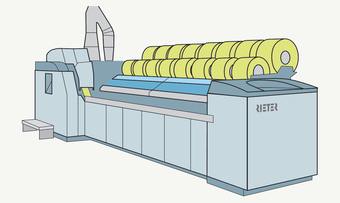
\includegraphics[width=0.5\textwidth]{Rieter_comber.jpg}
	\caption{Rieter Comber E86 (\cite{cite:RIKIpedia_combing})}
	\label{fig:rieterComber}
\end{figure}

It consists of three main parts: 
\begin{itemize}
	\setlength{\itemsep}{5pt}
\item The Feed

\item The Nipper

\item The Comb
\end{itemize}
%The process of removing the impurities is formed by attaching the input fiber in form of sliver to the feed roller
An input of this process is textile sliver (described in chapter \ref{textileFibers}).
\subsection{Spinning Process}
\label{spinningProcesses}
The term “spinning” in this context refers to the process that executes conversion of a large quantity of individual unordered fibers of relatively short length into a linear, ordered product of very great lengths by using spinning machines. There are three main methods of executing process of spinning:
\begin{itemize}
	\setlength{\itemsep}{5pt}
\item Ring Spinning,

\item Rotor Spinning and

\item Air-jet Spinning.
\end{itemize}
All of these systems yields yarn with different structures and properties. Each system has its advantages and limitations in terms of technical feasibility and economic viability.

\subsection{Wavelength}
In encylopaedia Britannica the \textit{wavelength} is defined as:
\textit{Distance between corresponding points of two consecutive waves.} \cite{cite:brittanicaWavelength}. In other words, wavelength is the spatial period of a sinusoidal wave. Under an assumption a wave is moving at a fixed speed, then frequency of the wave is inversely proportional to the wavelength. This is shown in a figure \ref{fig:wavelengthExplaination}.
\begin{figure}[h]
	\centering
	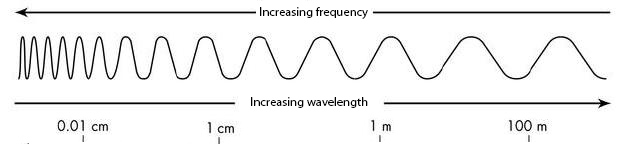
\includegraphics[width=0.7\textwidth]{wavelengt_explained.jpg}
	\caption{Wavelength}
	\label{fig:wavelengthExplaination}
\end{figure}

From the mathematical representation of the sinusoidal waves a formula can be derived that expresses relation of a wavelength, velocity and frequency of a wave, as can be seen in \cite{cite:fundamentalsOfPhysics}. The formula is stated as follows in \ref{eq:wavelengthFormula}.
\begin{equation} \label{eq:wavelengthFormula}
\lambda=\frac{v}{f}
\end{equation}

In the textile engineering this term is used to describe wave property of a textile fiber that is being processed. This can improve the perception of a quality by knowing the wavelength of a defect in the fiber \cite{cite:TextileEngineering}. In some book about textile engineering the term wavelength is interchanged with term \textit{cut length}. As an example, this is useful in situations such as when a textile defect has been found at the wavelength $\lambda=8cm$ and it allows to quickly visually check if any unwanted pattern with this wavelength is visible on the fiber.

\subsection{Coefficient of Variation}
\label{sec:CoefficientOfvariation}
Coefficient of variation, hereafter CV, is a measure of dispersion of a probability or frequency distribution. In textile engineering its used as indicator of quality of textile fibers, because as it states the irregularity of sampled length. Often it is expressed as percentage, which is noted as CV\%. It can be calculated according to the equation \ref{eq:CVCalculationIntroduction} \cite{cite:fundamentalsOfSpunYarn}.

\begin{equation} \label{eq:CVCalculationIntroduction}
 CV\% = \frac{\sigma}{\mu} \cdot 100
\end{equation}

\subsection{Variance-length Curve}
\label{sec:VarianceL_curve}
CV\% values for different wavelengths provides useful information of the variation of a fiber. When CV\% values of different wavelengths are simultaneously represented graphically, it provides the possibility of determining wavelengths at which defects occur and consequently identify the process stage that caused it. This graphical representation is called \textit{variance-length curve}.

\section{State of Art}
\subsection{Overview of Yarn Quality Sensors}
An importance of yarn quality on final product became clear in the 1950s when first electronic yarn quality sensors were invented. Since then many principles were used in the detection of yarn defects - optical, mechanical or even chemical \cite{cite:1}.

Sensors of yarn quality are in the textile industry often called \textit{yarn clearer}. This term was created for first such devices because goal of yarn clearers wasn't only to discover possible yarn defects but also to immediately remove them. Today, yarn clearers analyze defects that are much more complex (given their properties such as periodicity etc.) and difficult to be immediately removed. Such defects are invisible to a naked eye on single yarn and they appear only when turned to fabric.

The following overview is concerned with yarn quality sensors that have similar purpose and functions as the developed device. Therefore, only online yarn clearers that check quality of spun yarn on every spinning point in real-time are listed. All of the following devices are also aimed to be used on the yarn spun by a rotor spinners (see \ref{spinningProcesses}).

\subsubsection{Uster Quantum 3}
Uster Quantum 3 is modern yarn clearer, which provides detection of many types of defects and includes several interesting features:

\begin{itemize}
	\setlength{\itemsep}{5pt}
	\item full yarn body display,
	\item foreign matter sensor with multicolored light sources,
	\item polypropylene detection,
	\item detection of moiré,
	\item unevenness calculation CV\%,
	\item IPI classification,
	\item calculation of hairiness,
	\item spectrograms calculation.
\end{itemize}

Uster Quantum 3 has been developed by company Uster Technologies, which is developing yarn clearers for 30 years. Their devices often feature an application of new technologies and they offer high-quality products.

This yarn clearer is also one of the two commercially sold products capable of calculating spectrograms and evaluate yarn unevenness CV\%.

 


\section{Digital Signal Processing}
The largest part of work on this project is oriented on digital signal processing (DSP). Usage of modern advanced algorithms from this field allowed designing projected device in the first place. This section covers the most important algorithms that are used in this project.
	
	Digital signal processing is an area of science and engineering that has developed rapidly over the past 40 years as a result of significant advances in digital computer technology. Today, many of the signal processing tasks that were conventionally performed by analog means are now realized by less expensive digital hardware \cite{cite:2}.
	
	To perform the processing digitally, there is the need for the conversion between an analog signal and digital signal. This is done by an interface called analog-to-digital (A/D) converter, which yields a digital signal as it's output that is appropriate as an input to the digital processor \cite{cite:2,cite:3}.
	
\subsection{Discrete Fourier Transform}
\label{sec:DiscreteFourierTransform}
To perform frequency analysis on a discrete-time signal ${x[n]}$, we convert the time-domain sequence to an equivalent frequency-domain representation. This conversion is obtained by Discrete Fourier Transform that can be algebraically formulated as (according to \cite{cite:2,cite:3}).
	
Given N consecutive samples $x[n], 0 \leq n \leq N-1$ of a periodic or aperiodic sequence, the N-point Discrete Fourier Transform(DFT) $X[k], 0 \leq k \leq N-1$ is defined by
\begin{equation} \label{eq:DFT}
X[k]=\sum_{k=0}^{N-1}x[n]e^{-j \frac{2 \pi}{N} kn}.
\end{equation}
Given $N$ DFT coefficients $X[k], 0 \leq k \leq N-1$, we can recover the N sample values of sequence $x[n], 0 \leq n \leq N-1$ using Inverse Discrete Fourier Transform (IDFT) given by
\begin{equation} \label{eq:IDFT}
x[n]=\frac{1}{N} \sum_{k=0}^{N-1}X[k]e^{j \frac{2 \pi}{N} kn}.
\end{equation}
If $x[n]$ has infinite duration, the frequency samples  $X[2 \pi k/ N], k=0, 1, ..., N-1$ correspond to a periodic sequence $x_{p}[n]$ of period N, which is an aliased version of $x[n]$. When the sequence $x[n]$ has finite duration of length $L \leq N$, then  $x_{p}[n]$ is simply a periodic repetition of $x[n]$.

The DFT defined in (\ref{eq:DFT}) can also be rewritten as
\begin{equation} \label{eq:DFT2}
X[k]=\sum_{k=0}^{N-1}x[n]W^{kn}_{N},\; k = 0, 1, ..., N-1,
\end{equation}
where
\begin{equation} \label{eq:Twiddle}
W^{kn}_{N}=e^{-j \frac{2 \pi}{N} kn}=\cos(\frac{2\pi kn}{N})-j\sin(\frac{2\pi kn}{N}), \;0\leq k,n\leq N-1
\end{equation}
The parameters $W^{kn}_{N}$ are called the twiddle factors \cite{cite:RT_DSP}.
\par
Understanding properties of DFT is critical for application of the transformation to practical problems. List of the main DFT properties contains:
\begin{itemize}
	\setlength{\itemsep}{5pt}
\item Linearity,

\item Periodicity,

\item Complex Conjugate,

\item Circular Convolution,

\item DFT and the z-transform.
\end{itemize}
For detailed description of DFT properties see \cite{cite:2,cite:RT_DSP}.

The operation of selecting a finite number of samples called windowing is equivalent to multiplying the actual sequence $x[n]$ defined in a range $-\infty < n < \infty$, by a finite-length sequence $w[n]$ called window. Using simplest rectangular windowing (truncation) on a signal can cause an effect called \textit{leakage}, which transfers power from frequency bands that contain a large amount of signal power into bands that contain only a little. This may create "false" peaks, peaks at wrong frequencies or changes the amplitude of existing peaks. 

Another effect of time-windowing is \textit{smearing}. Which causes a spread of spectrum accordingly to the width of the mainlobe of the window spectrum. This result in loss of resolution \cite{cite:3} .
% Image according to ADSP 400/ obr 7.23

Therefore, a "good" window should have low-level sidelobes and a narrow mainlobe to minimize both of these effects. There are four most known windows used for time-windowing: 
\begin{itemize}
	 \setlength{\itemsep}{5pt}
\item Rectangular,
	
\item Triangular (or Bartlett),
	
\item Hann,
	
\item Hamming.
\end{itemize}	
Their differences (as shown in image XXX) relays in a different width of mainlobe and peak sidelobe level.
% Image according to ADSP 406/ obr 7.26 

%The length N of the DFT should be larger than L = T0/T to obtain good visual representation of DTFT. If we set N to power of two N=2^Q, fft calculation %done microcontroller is executed faster.
\subsection{Fast Fourier Transform}
\label{sec:FFT}
Difficulty in using the DFT for practical applications is its high computational requirements. Direct computation of the N-point DFT requires computational cost of $N^2$. However class of efficient DFT algorithms called \textit{Fast Fourier Transform (FFT)} has computational cost proportional to $Nlog_{2}N$ \cite{cite:RT_DSP,cite:3}.
\par 
Decimation-in-time FFT algorithms are based in splitting the N-point DFT summation into two summations, that one sum over the even-indexed points of $x[n]$ and another sum over the odd-indexed points of $x[n]$.
Therefore, we obtain
\begin{equation} \label{eq:decimInTime1}
\begin{aligned}
X[k] &= \sum_{n=0}^{N-1}x[n]W^{kn}_{N}, \; k=0,1,...,N-1\\
     &= \sum_{m=0}^{N/2-1}x[2m]W^{k(2m)}_{N} + W^{k}_{N}\sum_{m=0}^{N/2-1}x[2m+1]W^{k(2m)}_{N}
     \end{aligned}
\end{equation}
Dividing sequence $x[n]$ we get two shorter sequences:
\begin{equation} \label{eq:decimatedSequencesA}
a[n]=x[2n],\qquad n=0, 1, ..., N/2 -1
\end{equation}
\begin{equation} \label{eq:decimatedSequencesB}
b[n]=x[2n+1],\qquad n=0, 1, ..., N/2 -1
\end{equation}
Shorter sequences are obtained by \textit{decimating}
\footnote{Decimation of a signal with sampling rate $f_{s}$ by a integer factor $D$ results in the lower sampling rate $f'_{s}=f_{s}/D$.}
 the sequence $x[n]$, thus, this FFT algorithm is called decimation-in-time.
Substituting definitions \ref{eq:decimatedSequencesA} and \ref{eq:decimatedSequencesB} into \ref{eq:decimInTime1} yields
\begin{equation} \label{eq:fft2_A}
A[k]=\sum_{m=0}^{N/2-1}a[m]W^{km}_{N/2},\qquad k=0, 1, ..., N/2 -1
\end{equation}
\begin{equation} \label{eq:fft2_B}
B[k]=\sum_{m=0}^{N/2-1}a[m]W^{km}_{N/2},\qquad k=0, 1, ..., N/2 -1
\end{equation}
where $A[k]$ and $B[k]$ are $N/2$-point DFTs \cite{cite:3,cite:2}.

Thus, we can calculate $N$-point DFT $X[k]$ from the $N/2$-point DFTs $A[k]$ and $B[k]$ (\ref{eq:fft2_A}, \ref{eq:fft2_B}) using the following merging formulas
\begin{equation} \label{eq:fft3_A}
X[k]=A[k] + W^{k}_{N}B[k],\qquad k=0, 1, ..., N/2 -1
\end{equation}
\begin{equation} \label{eq:fft3_B}
X[k+\frac{N}{2}]=A[k] - W^{k}_{N}B[k],\qquad k=0, 1, ..., N/2 -1
\end{equation}
These formulas (\ref{eq:fft3_A}, \ref{eq:fft3_B}) can be applied to any FFT of even length \cite{cite:3}.

This procedure is shown in Figure XXX (\cite{cite:3}). The displayed structure in the figure is called the butterfly network. Each butterfly consists of just a single complex multiplication by the twiddle factor $W^{k}_{N}$, one addition and one subtraction. 

An example for $N=8$ is shown in Figure XXX. Each $N/2$-point DFT can be computed by two smaller $N/4$-point DFTs. By repeating the same process, we will obtain a set of two-point DFTs, which is illustrated in Figure XXX \cite{cite:RT_DSP}.

FFT algorithm \textit{decimation-in-frequency} is similar to the decimation-in-time, with important differences, that the decomposition and symmetry relationships are reversed. The bit reversal occurs at the output instead of the input and the order of the output samples $X[k]$ will be rearranged \cite{cite:RT_DSP}.

The FFT algorithms shown in the previous paragraphs can be modified to calculate the inverse FFT (IFFT).

\subsection{Power spectral density}
%Consider a signal $x[n]$ of length $N$ with DFT $X[k]$ 
Energy Spectral Density $S(\omega)$ defined as \ref{eq:EnergySD}
\begin{equation} \label{eq:EnergySD}
S(\omega)=\left|Y(\omega)\right|^2
\end{equation}
Which can be obtained from Parseval's theorem (\ref{eq:Parseval})
\begin{equation} \label{eq:Parseval}
\sum_{t=-\infty}^{\infty}\left|y(t)\right|^2 = \frac{1}{2\pi}\int_{-\pi}^{\pi}S(\omega)d\omega
\end{equation}
This equality shows that $S(\omega)$ represents the distribution of sequence energy as a function of frequency. For this reason, $S(\omega)$ is called the \textit{energy spectral density}. 
Most of the signals in practical applications are such that their variation in the future cannot be known. It is only possible to make probabilistic statement about the variation. Such sequences are called \textit{random signals}. 

A random signal usually has finite average power, therefore, we can use average power spectral density for its characterization. Which is, for simplicity, better known under name \textit{power spectral density} (PSD). As shown in \cite{cite:SAoS} is defined as
\begin{equation} \label{eq:PSD1}
\phi(\omega) = \sum_{t=-\infty}^{\infty}r(k)e^{-i\omega k}
\end{equation}
where $r(k)$ is auto covariance function $r(k) = E[y_{t}y_{t+k}]$.
The PSD is very useful in the analysis of random signals since it provides us with information about the distribution of the average power over the frequency. There are several different methods for estimating the PSD. 

Methods that require direct use of a finite signal for purposes of autocorrelation calculation are called \textit{non-parametric} methods. On the other hand, methods that rely on a model for signal generation are call \textit{parametric} methods \cite{cite:RT_DSP}. Widely used non-parametric methods are

\begin{itemize}
	\setlength{\itemsep}{5pt}
\item Bartlett method,
\item Blackman-Turkey method,
\item Welch method or
\item Danielle method.
\end{itemize}

They differ mainly in the resolution and variance level of the result. For a detailed description of methods see \cite{cite:2}.

\section{Digital Processing Techniques}

\subsection{Spectrograms}

\section{Embedded systems and microcontrollers}
There are many definitions of embedded systems. The one picked for this thesis subjectively seems well accurate in the description of the given term. It goes as follows.

\textit{"An embedded system is a specialized computer system that is usually integrated as part of a larger system. An embedded system consist of a combination of hardware and software components to form a computational engine that will perform a specific function. Unlike desktop systems which are designed to perform a general function, embedded systems are constrained in their application \cite{cite:SE_for_ES}."}

Embedded systems very often perform in reactive and real-time environments, which has to fulfill the real-time constrains that are described in \ref{R-T constrains}. Not satisfying these constraints can cause significant system consequences. If the consequences consist of a degradation of performance, but not a failure, the system is referred to as a soft real-time system (e.g. highway car counter). On the contrary, if the consequences are a system failure, the system is referred to as a hard real-time system (e.g. a braking system in a vehicle). 

Typical embedded system receives information about the surrounding environment via sensors and responds with actuators. General block diagram of such system is in Figure XXX.																	
\subsection{Embedded systems}

\subsection{DSP Hardware Options}
DSP algorithms can be implemented on different types of digital hardware. The following are the widely used options for DSP systems:
\begin{itemize}
	\setlength{\itemsep}{5pt}
\item Special-purpose chips such as application-specific integrated circuits (ASICs).
\item Field-programmable gate arrays (FPGAs).
\item General-purpose micro-processors or micro-controllers ($\mu$P/$\mu$C).
\item General-purpose digital signal processors.
\item DSP processors with application-specific hardware accelerators \cite{cite:RT_DSP}.
\end{itemize}

Each hardware (HW) platform has different advantages and constraints for different applications, thus, there is no \textit{best} HW platform that could be used for every practical project. Instead, each option should be carefully considered from point of flexibility, required design time, power consumption, performance and cost. 

Characteristic of mentioned hardware options are summarized in Table XXX (\cite{cite:RT_DSP}).

\subsection{Real-time constraints}
\label{R-T constrains}
Generally, a real-time system is one that must process information and produce a response within a specified time, else risk severe consequences, including failure. A real-time DSP system demands that the signal processing time $t_{p}$, must be less than sampling period $T$, that is
\begin{equation} \label{eq:hardRealTime1}
t_{p}+t_{o}<T,
\end{equation}
where $t_{o}$ is overhead time of input-output (I/O) processing.
Thus, this limitation gives constraint to the highest frequency signal that can be processed by DSP systems in sample-by-sample processing, given as

\begin{equation} \label{eq:hardRealTime2}
f_{M} \leq \frac{fs}{2} < \frac{1}{2(t_{p}+t_{o})} \cite{cite:RT_DSP}.
\end{equation}

Using different techniques of processing can reduce the I/O overhead time and increase the performance of the DSP hardware platforms. For example by applying a block-by-block processing, where the I/O operations are handled by DMA controllers, which place data samples in memory buffers \cite{cite:RT_DSP}.

Today, with performance improvement of hardware platforms, it is even possible to calculate FFT (see \ref{sec:FFT}) of 64-points in a matter of tenths of milliseconds with low-cost ARM microprocessor (e.g. specifically in $0.16 ms$ for microcontrollers of STM32F1xx series according to \cite{cite:STM32_DSP_library}).
\subsection{ARM Cortex-M3}
\label{sec:ARM_M3}
First manufactured microprocessor of Cortex series was ARM Cortex-M3. It was developed in 2006 and its target group of application was 32-bit microcontrollers. Its main advantage is an excellent efficiency which yields high performance and a low energy consumption without the need for a very high system clock frequency. It is based on architecture \textit{ARMv7}.

An ARMv7 architecture was developed as a modern type of a general architecture that could be used for low-level microprocessors as well as for high-performance application processors. Design of the architecture is split into three main profiles:
\begin{itemize}
	\setlength{\itemsep}{5pt}
	\item Profile A - aimed at application processors for performance-intensive systems capable of using embedded operational systems (such as Symbian, Android or Linux Embedded).
	\item Profile R - aimed at high-performance processors for real-time applications.
	\item Profile M - aimed at wide-range processors for deeply embedded applications \cite{cite:ARM-M3}.
\end{itemize}

\subsubsection{Instruction Set}
There are two instruction sets supported by ARM cores in general: the ARM instructions which are 32-bit and the Thumb instructions which are 16-bit. During the execution, the processor can switch either to the ARM state or to the Thumb state accordingly to the instruction set it is currently using.

The ARMv7 architecture is using new instruction set called a Thumb-2 which consists of the 32-bit Thumb instructions and also 16-bit Thumb instructions. This yields big improvement from the perspective of the ease of use, performance and code size. It allows execution of a complex operation in state Thumb which increases the effectivity \cite{cite:ARM-M3}.

\chapter{Practical Implementation}
Prior to the design of the system architecture, a list of requirements for the device had to be created. This was done in discussion with company Rieter CZ s.r.o. who provided resources for development. The most important requirement is that the device shall be able to analyze the quality of a yarn and sliver. This separates the project in two parts, where core software algorithms are shared but other parts significantly different. 

\section{Sliver Quality Analysis}
 The sliver quality analysis requires development of software and also additional hardware. In this case - opposite to yarn quality system - it is necessary to design new processing board due to the fact that sliver and yarn have significant size differences (see \ref{textileFibers} and different sensors need to be used). Also, it was decided that device developed in this project will be only prototype version, thus, it has additional functionality that can be removed in a final product. The main requirements and features for the device prototype were defined as follows:
\begin{itemize}
	\setlength{\itemsep}{5pt}
	\item The device shall be able to measure the diameter of a sliver.
	\item The device shall be able to filter, and process measured data in a way that allows calculating CV\% value and Variance-length Curve.
	\item The device shall be able to measure the diameter with one or more specified sensors simultaneously.
	\item The device shall be able to send measured data to the service computer in real-time.
	\item A PC application shall be implemented for receiving and storing data received from the device.
	\item The device shall be able to send measured data to the service computer in real-time.
	\item The device shall run on ARM microcontroller STM32F446.
\end{itemize}
\subsection{Hardware}
The purpose of the hardware section relays in providing the correct supply to the control unit and the sensors. Another feature of the hardware platform is processing the signals from sensors and converting it to the range which is suitable for ADC\footnote{Analog to digital converter} unit. Additionally, the hardware platform allows communicating with other distributed systems or PC by providing necessary interfaces. 

As the main innovation and focus of this project is oriented on the software, the hardware layout of PCB\footnote{Printed circuit board} was designed in Rieter according to the submitted electronic diagram. Resulting hardware platform is shown in figure \ref{fig:cvBox_dps}.

The hardware block diagram of the system is shown in Figure \ref{fig:blockDiagram_HW}. Description of each block follows in next paragraphs.
\begin{figure}[h]
	\centering
	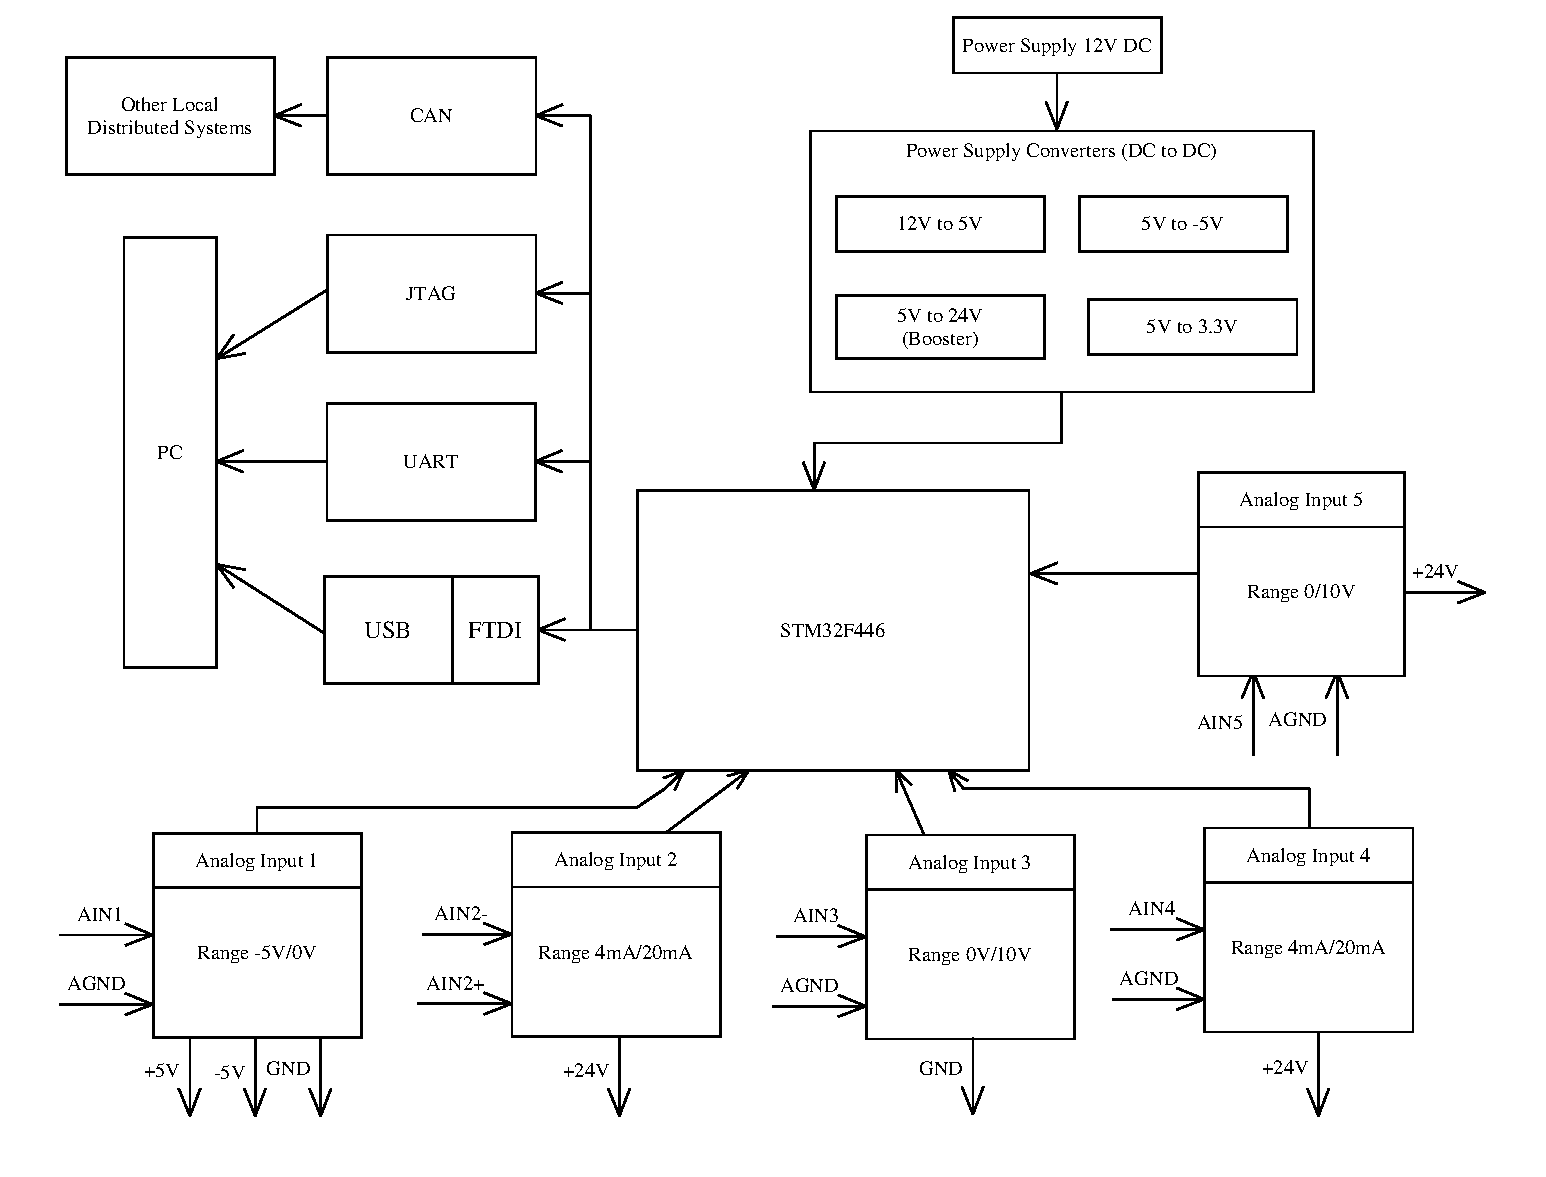
\includegraphics[width=1.0\textwidth]{blockSchematic5.eps}
	\caption{Block Diagram of the System}
	\label{fig:blockDiagram_HW}
\end{figure}

\begin{figure}[h]
	\centering
	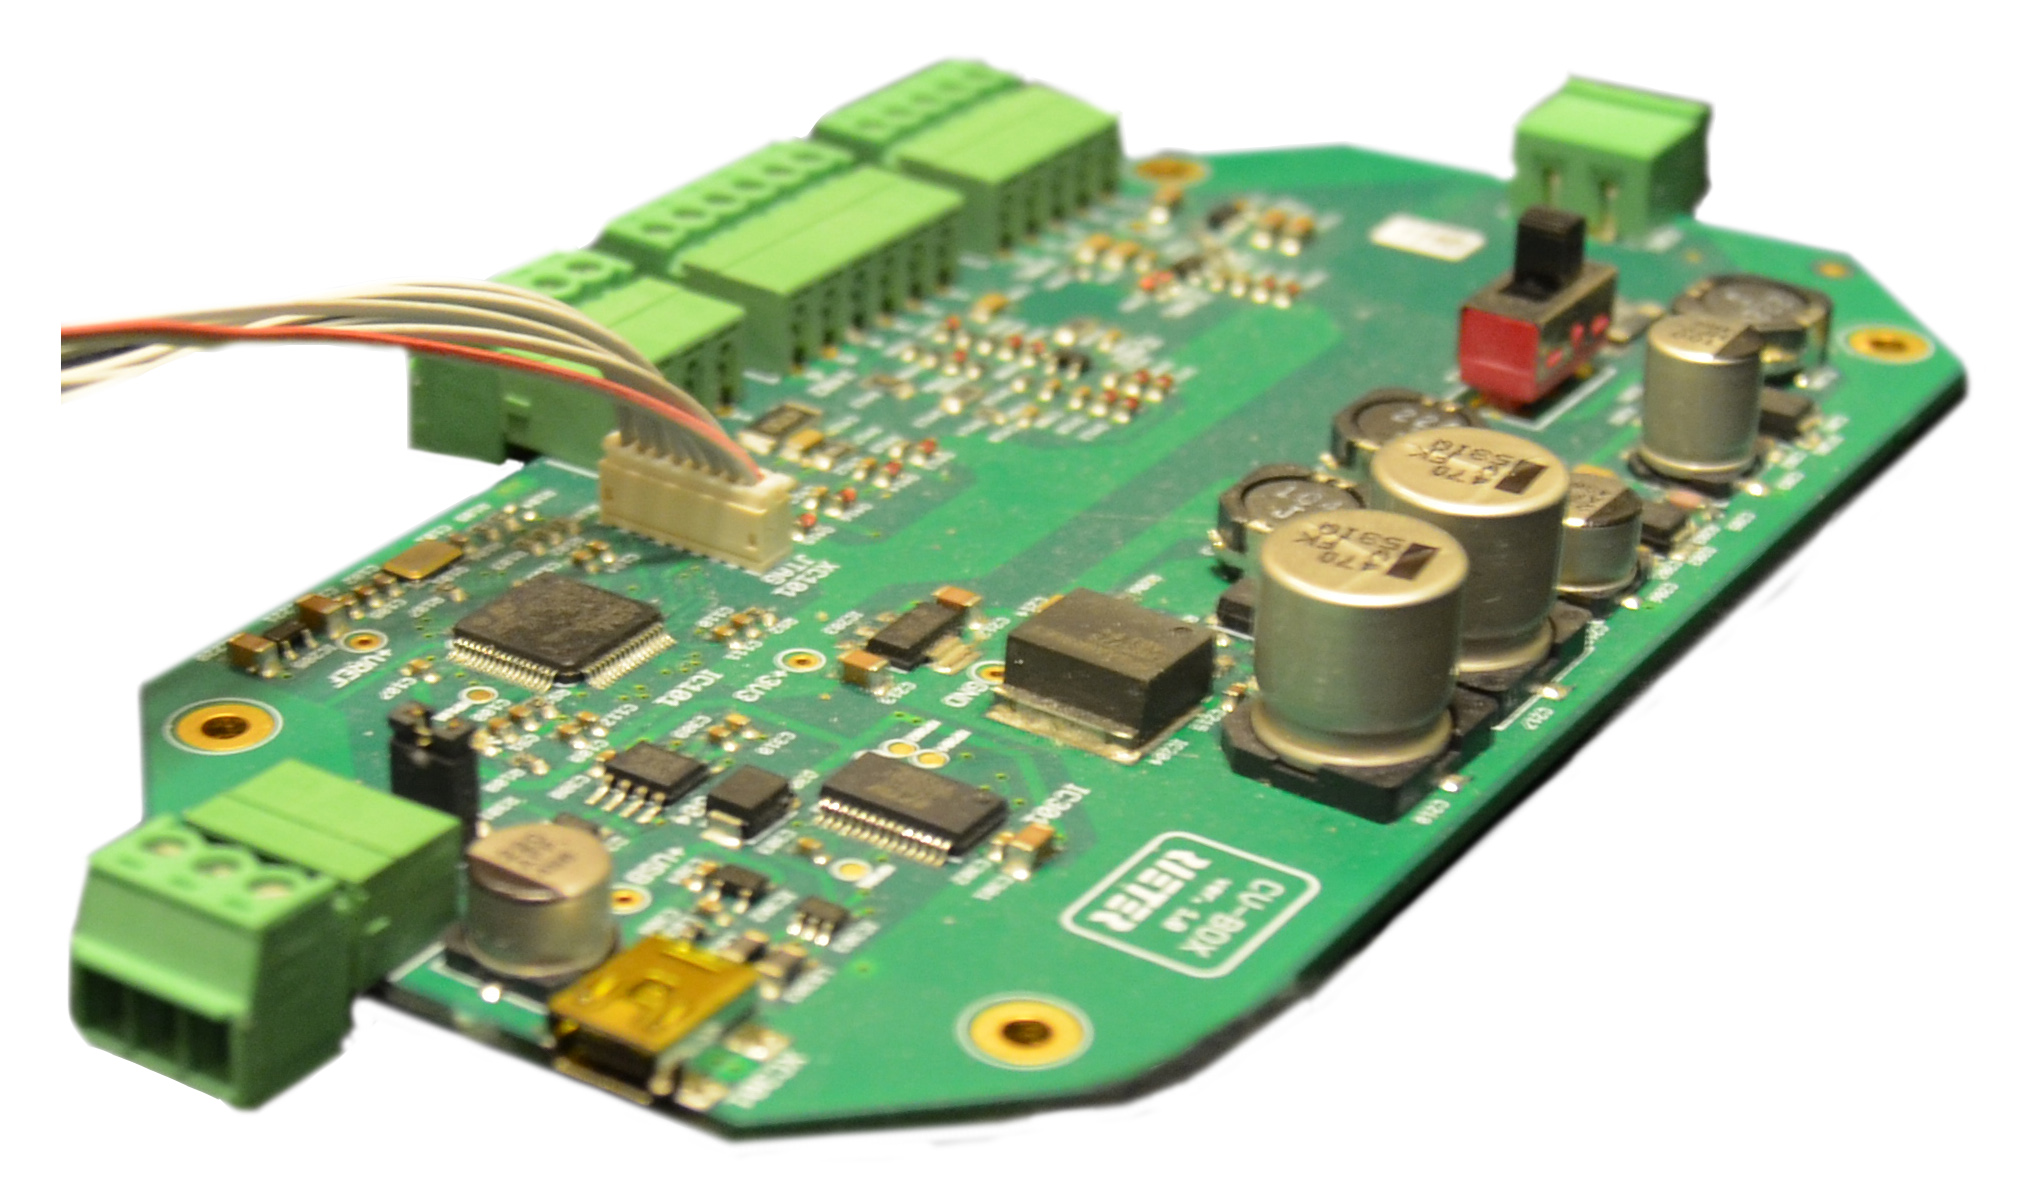
\includegraphics[width=0.75\textwidth]{cvBox.jpg}
	\caption{Hardware Platform - PCB}
	\label{fig:cvBox_dps}
\end{figure}

\subsubsection{Control Unit}
\label{sec:microController}
	The main part of the hardware is ARM microcontroller STM32F446 from STMicroelectronics. Its choice was given by a requirement from Rieter CZ s.r.o with a description that it was chosen for its low cost, sufficient performance and company's good long-term experience with manufacturer's support. 
	
	Microcontroller STM32F446 is based on ARM Cortex-M4 technology with ARMv7 architecture \ref{sec:ARM_M3}. With DSP instructions, it is capable of handling DSP algorithms such as FFT calculation in very short time (less than $0.5 ms$ for 1024-point FFT). Maximal operation frequency is $180 MHz$ at which gives $225 DMIPS$ (Dhrystone benchmark). The most important features and peripherals of this microcontroller are:
\begin{itemize}
	\setlength{\itemsep}{5pt}
	\item ARM 32-bit Cortex-M4, 180 MHz,
	\item 512 kB of Flash memory,
	\item 128 kB of SRAM,
	\item SWD and JTAG debug interface,
	\item 17 Timers and 3 ADC,
	\item Communication interfaces such as USART, CAN, SPI, SAI, SDIO, I2C, LIN etc.
\end{itemize}	
\subsubsection{Power Supply Converters}
Hardware platform of this system has to provide correct supply voltages to microcontroller and sensors. Supplying the sensors is especially complicated since they require three different voltages:
\begin{itemize}
	\setlength{\itemsep}{5pt}
	\item $5 V$,
	\item $-5 V$,
	\item $24 V$.
\end{itemize}
Voltage supply of the microcontroller is $3.3 V$.

The power supply of the hardware board was required to be $12 V$. Therefore, four DC-DC converters has to be designed, specifically:
\begin{itemize}
	\setlength{\itemsep}{5pt}
	\item $12 V$ to $5 V$,
	\item $5 V$ to $-5 V$,
	\item $5 V$ to $24 V$,
	\item $5 V$ to $3.3 V$.
\end{itemize}

For the first conversion from $12 V$ to $5 V$ was used an integrated step-down voltage regulator LM2594. To obtain $-5 V$ a charge pump inverter TPS60400 was used. The conversion from $5 V$ to $3.3 V$ is done by simple linear regulator MCP1825. The only step-up was necessary to get $24 V$ from $5 V$, for this purpose was chosen step-up voltage regulator LM1577.

Concrete circuits schematics of these converters are added as an attachment to the CD annexed with this thesis.

\subsubsection{Sensors and Input Modules}
\label{sec:Sensors}
To evaulate quality of a sliver, it is necessary to measure diameter of the sliver. For this a special sensors must be used. 
As can be seen in \ref{fig:blockDiagram_HW} the hardware platform contains 5 input modules. This was as an requirement from Rieter for the first version of the device, because in time of the development it was unsure which sensor would be used. Goal of each of the input modules is to convert the signal from connected sensor to such a voltage, which is in appropriate range for the ADC peripheral. Thus, the output voltage of each input module must be in range from $0$ to $2.8V$.

There was possibility of using capacitive sensor Mini Uster MS120. This is special type of a sensor capable of determining the diameter of a sliver. Output of the sensor is analogous and the voltage values are in range $0$ to $-5V$. It provides required specifications but has significant disadvantages. Since it is based on capacitive principle moisture of a measured sliver can influence the result. Sensor is also available only for higher price than would be suitable to meet the budget requirements. Sensor is designated to be connected into input module 1, which can handle the corresponding output voltage range.

Another possible sensor for measuring the diameter was Baumer Inductive Sensor S35A. This sensor measures distance and not the diameter itself. Thus, additional mechanical parts are necessary for its usage. It can be used in a way where a distance from the sensor to a roller, which is pressed to the sliver by a spring. If the sliver is thicker, the roller gets pushed closer to the sensor. This principle is shown in a figure \ref{fig:inductiveSensorDiagram}.
\begin{figure}[h]
	\centering
	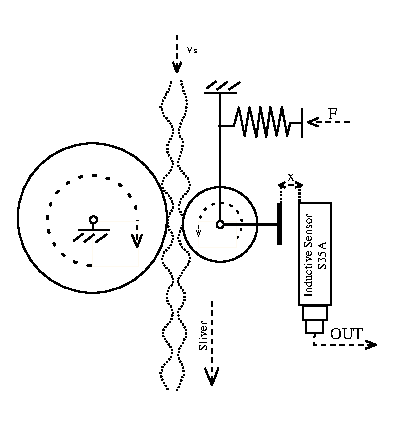
\includegraphics[width=0.65\textwidth]{SensorDiagram.eps}
	\caption{Usage of distance inductive sensor S35A for measurement of sliver diameter}
	\label{fig:inductiveSensorDiagram}
\end{figure}
Sensor is designated to be connected into input module 4, which was designed according to technical specifications from \cite{cite:InductiveSensor}:
\begin{itemize}
	\setlength{\itemsep}{5pt}
	\item Measuring distance: $0$ to $4mm$
	\item Resolution: less than $0,005 mm$
	\item Linearity Error: $\pm4\%$
	\item Temperature Drift: $\pm4\%$
	\item Response Time: less than $2ms$
	\item Current Output: $4$ to $20mA$
	\item Voltage Supply Range: $15$ to $30V$	
\end{itemize}
The sensor itself is shown in \ref{fig:sensor_only} (from \cite{cite:InductiveSensor}) and its application in a combing machine with additional mechanical parts for its usage is in \ref{fig:sens_Mechanical}.

\begin{figure}
	\centering
	\begin{subfigure}{0.5\textwidth}
		\centering
		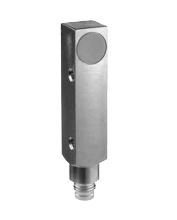
\includegraphics[width=0.75\linewidth]{baumer_inductiveSensor.JPG}
		\caption{Baumer Inductive Sensor S35A (\cite{cite:InductiveSensor})}
		\label{fig:sensor_only}
	\end{subfigure}%
	\begin{subfigure}{0.5\textwidth}
		\centering
		\includegraphics[width=1.0\linewidth]{Sensor_mechanics.jpg}
		\caption{Sensor application in a combing machine}
		\label{fig:sens_Mechanical}
	\end{subfigure}
	\caption{Variance-length curves}
	\label{fig:sensor_double}
\end{figure}

The project management from Rieter decided that the the Baumer Inductive Sensor S35A would be used as primary sensor in the first version of the device. Thus, hereafter using the term sensor refers to this particular inductive sensor.

Other input modules were added to the hardware platform to ensure that if new sensor could be obtained, then there would be a possibility to connect it to the device.

\section{Algorithm for Sliver Quality Analysis}
\label{algorithmForSliver}
Algorithm overview diagram is shown in Fig. \ref{fig:software_overview}. This is the simplified representation of software used for sliver quality analysis in the microcontroller. The input of the system is a sample - measured by ADC - which represents the diameter of the sliver. Required output shall be a variance-length curve which is composed of CV(\%) values calculated for several wavelengths\footnote{\label{footnote1:textileTerms}For explanation of the terms used in this paragraph see chapter XXX}. Each software components are individually described in following paragraphs.

The main principle of designed quality analysis lies in determining the coefficient of variation (CV(\%)) value. This value can be obtain from signal that corresponds to appropriate wavelength (cut length). Different wavelengths can be yielded by filtrating the input signal with lowpass filter that passes only frequencies that correspond to given wavelength. Specifically if it is chosen that signal of wavelengths between $\lambda_{min}$ and $\lambda_{max}$ is required, then signal can contain the frequencies only up to $f_{max}$. Where relation between $\lambda_{min}$ and $f_{max}$ is based on knowledge of the \textit{sliver speed} $v_{s}$\footnote{Speed of winding up sliver during the process of combing.} determined as follows in equation \ref{eq:wavelengthToFreq}:

\begin{equation} \label{eq:wavelengthToFreq}
f_{max} = \frac{v_{s}}{\lambda_{min}}.
\end{equation}

From this, we can see that the lower boundary $\lambda_{min}$ is more important and as a matter of notation it is used to specify the whole wavelength range. This means that when speaking of CV(\%) for the wavelength of $\lambda$ it is actually meant $\lambda_{min}$.

When sufficient amount of CV(\%) values for different wavelength is obtained, then they are joined in \textit{variance-length curve} (see chapter XXX). This curve can be easily represented graphically and as such it allows users to see the quality of a sliver for different wavelengths just by looking at the shape of the curve. Taking new samples may cause a change in appropriate CV(\%) values, therefore, the variance-length curve is periodically updated. It is important to mention that part of the curve with the lowest wavelength can be updated several times before even one update of higher wavelengths can be calculated. This is due to the fact that higher wavelengths require significantly more input samples.

\begin{figure}[h]
	\centering
	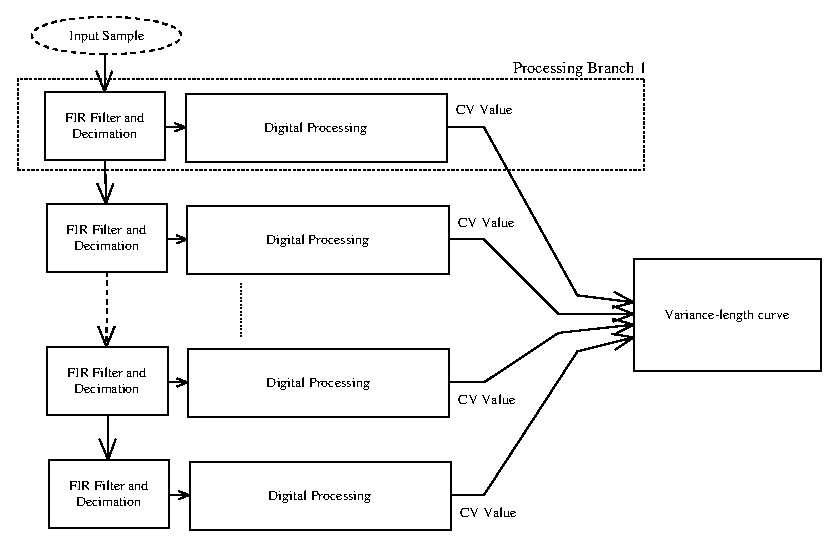
\includegraphics[width=1.0\textwidth]{system_overview.eps}
	\caption{Software Architecture Overview}
	\label{fig:software_overview}
\end{figure}

\subsection{Solution for Embedded Systems Constraints}
\label{sec:SolutionForEmbedded}
As described in chapter \ref{R-T constrains} using embedded systems brings several important constraints. The most significant issues this system has to solve were DSP performance and memory restriction of used microcontroller. The memory issue turned to be critical, because if we had control unit capable of storing hundreds of thousands of 16bit samples, we could easily store enough of input samples that allow calculation of all chosen wavelengths and then sequentially use low pass filter to obtain corresponding CV(\%) values. 

This could be done with a computer and was used in first version algorithm programmed in MATLAB. However, porting software to the microcontroller requires usage of decimation (see chapter XXX) which allows us to the lower number of samples used for each stage by throwing out every M-th sample (M is called the decimation factor). Of course, to prevent an \textit{aliasing}\footnote{Effect of violating the Nyquist-Shannon theorem.} low pass filter has to be used to filter out frequencies higher than \textit{Nyquist frequency}\footnote{Half of the sampling frequency}. But, as mentioned in previous paragraphs our application requires the use of low pass filter which will always filter out frequencies higher than Nyquist frequency. Thus, no other filter is required prior decimation.

Another issue is limitation of microcontroller because the DSP function for calculation of radix-4 FFT: \textit{cr4\_fft\_1024\_stm32} requires maximally 1024 samples as input. This disallows usage of FFT on a much larger amount of samples and processing its frequency spectrum in a way that would also provide us information on the quality of sliver, since (with enough samples) all required frequencies - corresponding to wavelengths - would be visible. This issue is also resolved by the decimation of the signal and using multi-rate analysis. 

Using this solution means that only buffers for 1024 samples are needed. Specifically one for each stage of calculation.

\subsection{Wavelengths Specification}
\label{sec:WavelengthSpecification}
One of the requirements for the software was determined that the device has to be capable of evaluating the quality of a sliver for wavelengths in the range from $0.25 cm$ to $512 cm$ because others wavelengths are not significant enough to the final product. This range is then divided among twelve values, each wavelength representing one stage of calculation. This division will yield each wavelength to be the double of the previous and that allows us to set the decimation factor (see \ref{sec:SolutionForEmbedded}) to $M=2$ for decimators in all stages. The table XXX shows these wavelengths and their corresponding sampling frequencies $f_s$ calculated according to equation \ref{eq:wavelengthToFreq} with sliver speed $v_{s}=30 cm/s$. 

This sliver speed was chosen as it is default settings of combing machines and was used during testing. If different sliver speed is set on combing machine, its value is sent over a CAN communication during initialization and the basic sampling frequency is adjusted in a way that decimation factor always stays set on $M=2$. This allows using the same filter coefficients independently on value of sliver speed.

Knowing this information allows us to determine a \textit{cut off frequency}\footnote{XXX} $f_c$ of FIR filters that are used for limiting the bandwidth and an anti-aliasing. This is done according to the formula $f_c=f_s/2$ for each wavelength as shown in table \ref{tab:Wavelengths}.

\begin{table}[htbp]
	\centering
	\caption{Wavelengths and corresponding frequencies}
	\begin{tabular}{crrrrr}
		\toprule
		Index of Stage & $\lambda_{min} [cm]$ & $\lambda_{max} [cm]$ & $\lambda_{s} [cm]$ & $f_s [Hz]$ & $f_c [Hz]$ \\
		\midrule
    1     & 0,25  & 0,5   & 0,125 & 240   & 120 \\
    2     & 0,5   & 1     & 0,25  & 120   & 60 \\
    3     & 1     & 2     & 0,5   & 60    & 30 \\
    4     & 2     & 4     & 1     & 30    & 15 \\
    5     & 4     & 8     & 2     & 15    & 7,5 \\
    6     & 8     & 16    & 4     & 7,5   & 3,75 \\
    7     & 16    & 32    & 8     & 3,75  & 1,875 \\
    8     & 32    & 64    & 16    & 1,875 & 0,9375 \\
    9     & 64    & 128   & 32    & 0,9375 & 0,46875 \\
    10    & 128   & 256   & 64    & 0,46875 & 0,234375 \\
    11    & 256   & 512   & 128   & 0,234375 & 0,1171875 \\
    12    & 512   & 1024  & 256   & 0,1171875 & 0,05859375 \\

		\bottomrule
	\end{tabular}%
	\label{tab:Wavelengths}%
\end{table}%

\subsection{Processing Branch}
CV values for each of these wavelengths (as shown in table \ref{tab:Wavelengths}) are calculated in individual processing branch. They are in sequential order and input for each branch is a partial result of the previous one.

With every sampling period, one sample is taken by ADC peripheral and its values are stored in memory by DMA\footnote{Direct Memory Access peripheral} and an interrupt is invoked. Then, in the interrupt handler a volatile flag determining that new sample was taken is set and main software state machine periodically checks its state. If the flag is set, the state is changed to first processing branch and sample processing begins.

Individual processing branch can be represented in the component diagram as shown in \ref{fig:singleBranch}.

\begin{figure}[h]
	\centering
	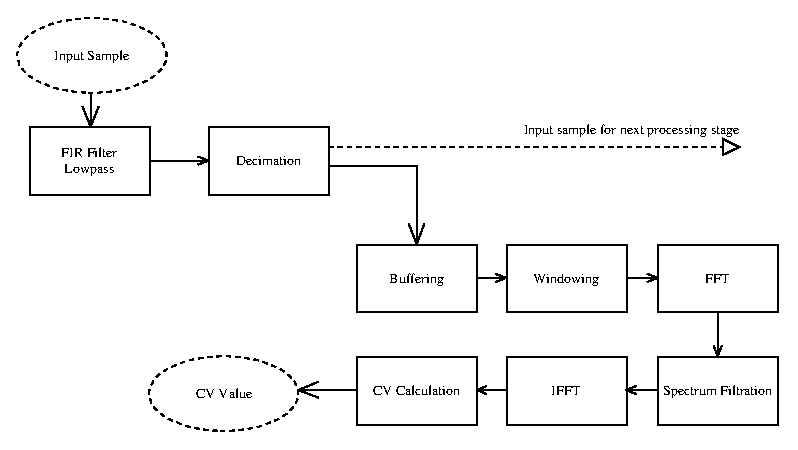
\includegraphics[width=1.0\textwidth]{sliver_singleBranch.eps}
	\caption{Component Diagram of Individual Processing Branch}
	\label{fig:singleBranch}
\end{figure}

Following paragraphs contain detail description for each component of processing branch.

\subsubsection{Input Sample}
Input sample is taken by ADC peripheral of the microcontroller. Particular input pin of ADC is set during initialization phase to the input module that is connected to the mechanical sensor of diameter (see \ref{sec:Sensors}). This sensor was chosen as for the first manufactured version of the device, because of its sufficiently accurate results and significantly lower price than other types of possible sensors. The ADC itself is set in DMA mode, with enabled interrupt after one sample is stored by DMA and to 12b size of the sample.
The sampling frequency is set to be the double of the frequency required for the first wavelength $\lambda=0.25 cm$. This frequency is dependent on sliver speed which is sent over a CAN communication during initialization. Adjusting the sampling frequency is the only solution that allows using the same filter coefficients independently on a value of the sliver speed. It is done by changing settings of the ADC peripheral.

\subsubsection{FIR Filter and Decimation}
\label{FIR filter}
Each branch has to contain lowpass FIR filter because it is necessary to prevent aliasing and to remove frequencies that correspond to the smaller wavelengths. As mentioned in \ref{sec:SolutionForEmbedded} each branch also has to implement decimation. Both of these operations can be combined in a component called \textit{FIR decimator}. This is an implementation of FIR filter that calculates only each $M-th$ output, where $M$ is a decimation factor. Thus, FIR decimator reduces required computational resources. 
The last version of DSP library for ARM microcontrollers does contain functions for the execution of FIR decimation. Unfortunately, these are not appropriate to use in this algorithm, since we need to the sample-by-sample filtration. This means that input for our implementation of FIR decimator has to be only one sample and output as well only one (or none) sample. Implementation is shown in the flowchart diagram \ref{fig:FIR_decimator}.

Input sample for the FIR decimator is added to the Input Buffer. This buffer is unique for each stage. First, algorithm checks whether Input Buffer already has at least 33 samples, which is a number of taps in used FIR filter (also number of filter coefficients). If there are 33 samples, first filter output can be calculated. If there are fewer samples (it never can be more) than 33, buffer index is iterated by one and function returns $-1$ which indicates that output sample is not ready.

Next, the decimation flag is checked. In case, it is false no output is required during this run of FIR decimator. But it is still necessary to shift the Input Buffer to the left so that the actual input sample is correctly used in next filter calculation. In opposite case, when it is true, this run should calculate and return the output value. This is the decimation part of the algorithm. The flag is negated after each valid output value is produced and this yields downsampling with factor $M=2$.

Output itself is calculated as a sum over the result of multiplication of Input Buffer and coefficients. This value is returned from the function that implements this filtering and is passed to other components in processing branch and to the next stage FIR decimator.

\begin{figure}[h]
	\centering
	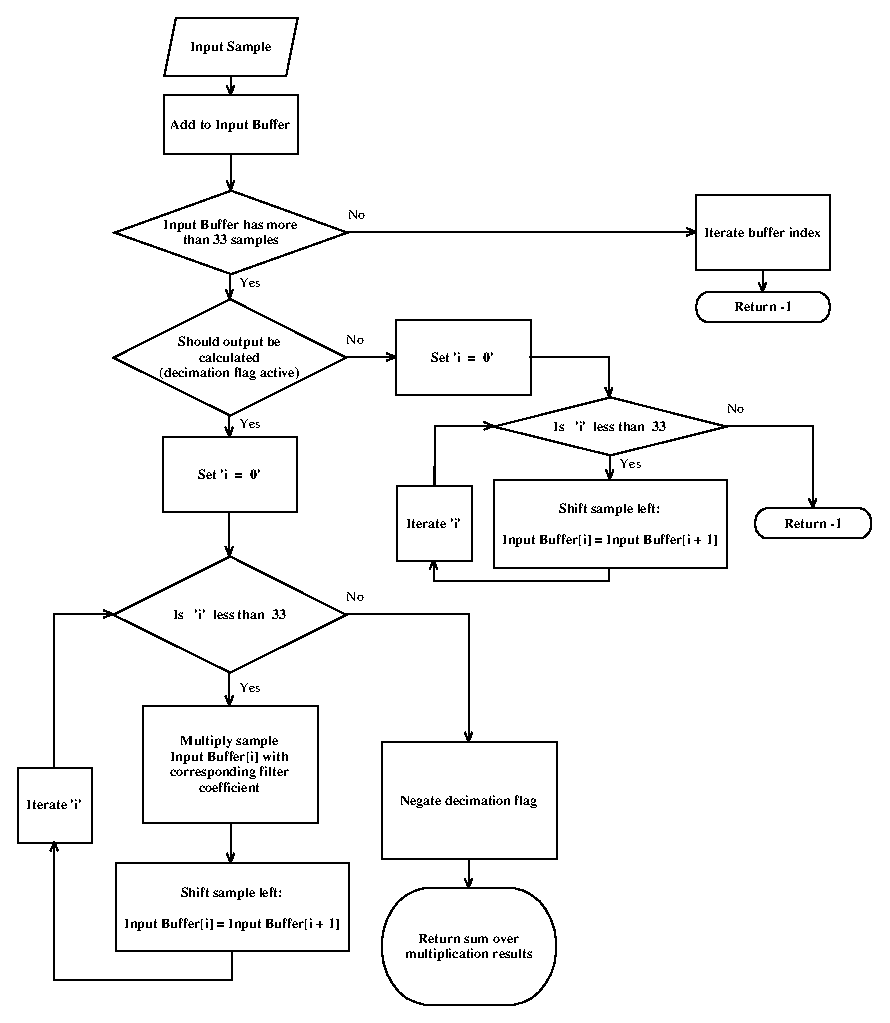
\includegraphics[width=1.0\textwidth]{firDecimator.eps}
	\caption{Flowchart diagram of FIR decimator component}
	\label{fig:FIR_decimator}
\end{figure}
FIR filter used in the FIR decimation was chosen as lowpass filter with order 32 and \textit{Bartlett-Hanning} window. Using this order and window yields required frequency properties as can be seen in its frequency response shown in figure \ref{fig:MagnitudeResponse}. Also its order is still small enough to allow sufficiently fast calculation. The cut-off frequencies are shown in table \ref{tab:Wavelengths}. The cut-off frequency is the same in normalized frequency\footnote{Range 0 to 1 and 1 corresponds to the $f_s/2$} for all the branches. Therefore, the same filter coefficients can be used for all the processing branches.
\begin{figure}[h]
	\centering
	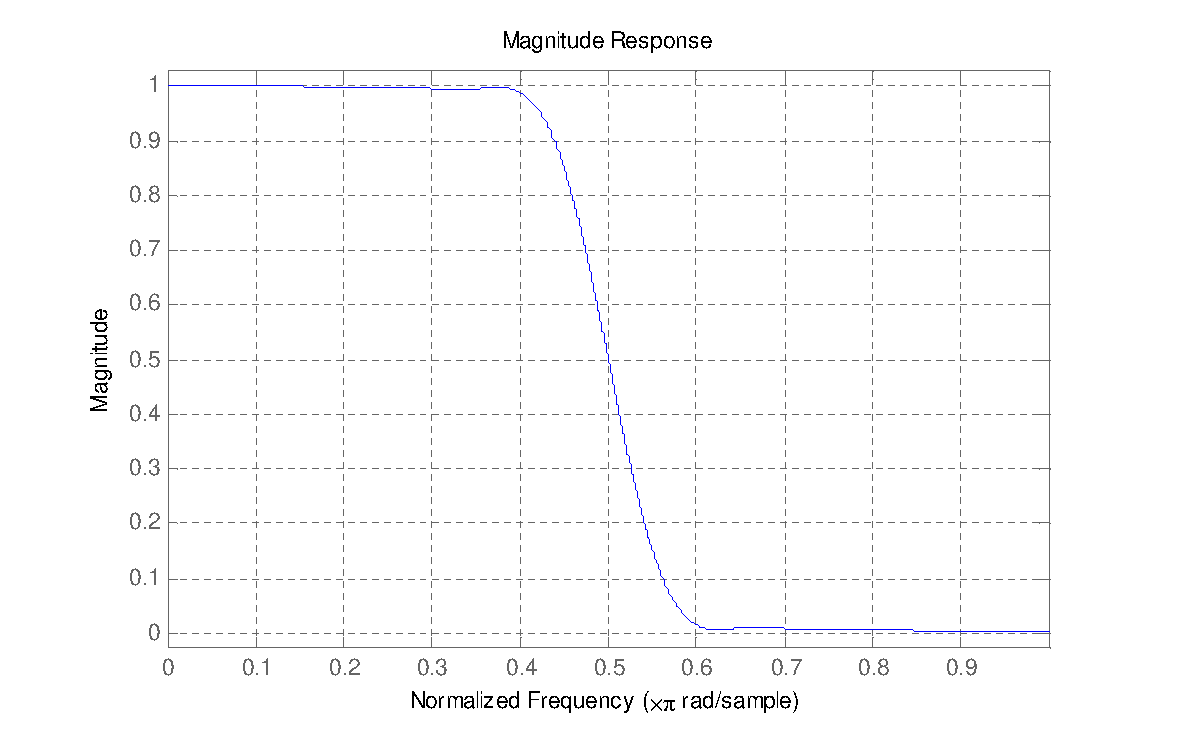
\includegraphics[width=1.0\textwidth]{magnitudeResponse.eps}
	\caption{Magnitude response of designed FIR filter}
	\label{fig:MagnitudeResponse}
\end{figure}

\subsubsection{Buffering}
Output samples from FIR decimator are buffered in vectors of length 1024. When the buffer is filled to full an appropriate flag is set and calculation can proceed to the next component. This creates a requirement for memory space. We know that it is required to has 12 processing stages and each stage has to have one buffer of 1024 sample and one sample is stored in 2B integer word. Another buffer for 1024 samples has to be ready for an output of FFT. From this conclude that \textit{Memory required} $= 12 \cdot 2 \cdot(1024 \cdot 2)=49152B\cong49.2kB$. This is not an issue for used microcontroller STM32F446 which has 128 kB of SRAM (see \ref{sec:microController}).

\subsubsection{Windowing}
Before calculation of FFT can be executed an operation called windowing (see chapter \ref{sec:DiscreteFourierTransform}) should be performed. This will prevent leakage and smearing, which are effects that are distorting the frequency spectrum obtained by FFT.

\subsubsection{FFT}
The frequency spectrum is obtained by algorithm called FFT (see chapter \ref{sec:FFT}). This is a fast implementation of Fourier transform and it is the most widely used technique used for obtaining frequency spectrum of signals. DSP libraries for ARM systems do contain functions for complex and real FFT. For our case we can use real FFT function \textit{arm\_rfft\_fast\_f32} with length of FFT 1024. This calculation can be performed on used microcontroller in tenths of milliseconds. \cite{cite:STM32_DSP_library}.

The FFT is defined over complex data but in many applications is the applied input real. Real FFT algorithms have speed advantage over complex algorithms of the same length because they properly use the symmetry properties of the FFT.

\subsubsection{Spectrum Filtration}
\label{sec:spectrumFiltration}
With frequency spectrum of the signal we can filter out the frequencies that are proclaimed as artefacts. Such errors in signal are caused by used mechanical sensor. This sensor measures the diameter of a sliver but during the measuring it is affected by mechanical vibration caused by turning gears inside the combing machine. Each of this gear creates vibration with frequency that is depending on a number of teeth and shaft speed. 

It would be possible to determine the frequencies that are distorting the signal from a detailed technical materials about combing machine and its gears. But unfortunately non such materials were available. Therefore, different approach to determine the error frequencies had to be used. 

For this purpose, a special measurement was executed (see chapter \ref{sec:MeasurmentAndTesting}). In this measurement it was possible to run the combing machine without any sliver, thus, only the mechanical vibrations were measured by sensor. Signal from this case was digitally post-processed in MATLAB and from obtained frequency spectrum specific artefact frequencies were distinguished. They were clearly visible even to the naked eye as the given frequencies had much higher amplitude than their surrounding. To obtain concrete frequency bins a peak detection was implemented and used. Result is shown in frequency spectrum of a signal measured without sliver with sampling frequency $f_s=240Hz$ (see figure \ref{fig:withoutMat_foundPeaks}).

\begin{figure}[h]
	\centering
	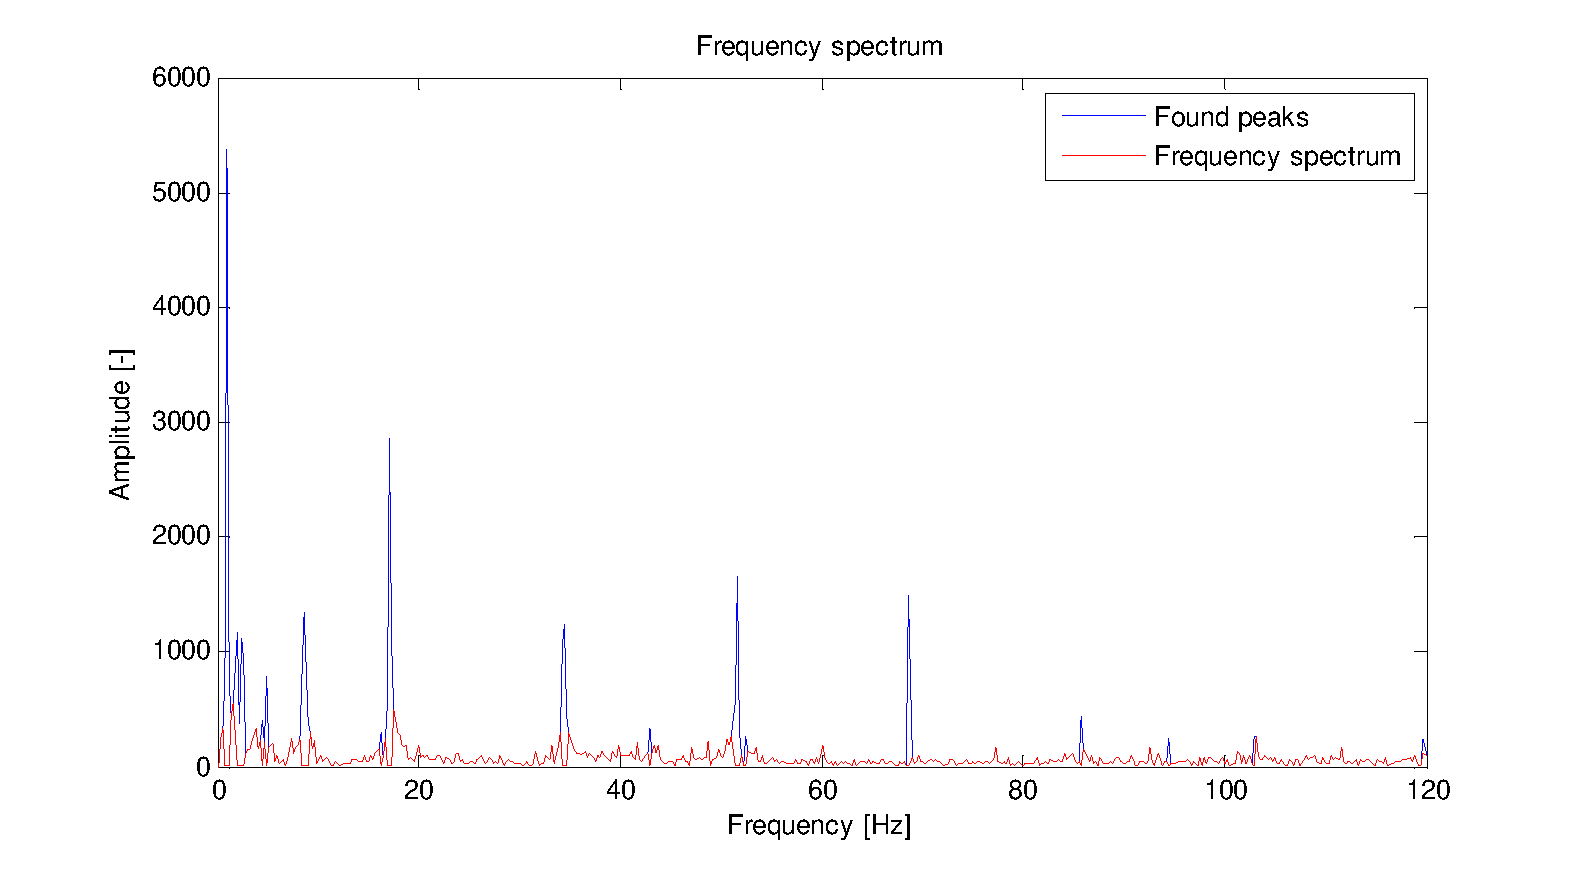
\includegraphics[width=1.0\textwidth]{withoutMat_foundPeaks_half.eps}
	\caption{Frequency spectrum of signal measured without sliver}
	\label{fig:withoutMat_foundPeaks}
\end{figure}

The most significant found frequencies are listed in table 	\ref{tab:DistortinFreq}%as follows.
\begin{table}[htbp]
	\centering
	\caption{List of distorting frequencies}
	\begin{tabular}{crrrrrrrrr}
%		\toprule
%		 & $\lambda_{min} [cm]$ & $\lambda_{max} [cm]$ & $\lambda_{s} [cm]$ & $f_s [Hz]$ & $f_c [Hz]$ \\
		\midrule
		Frequency [Hz]  & 0.94  & 1.88   & 2.34 & 4.45   & 4.92  & 8.672  & 17.11   & 34.45 & 42.89 \\
				
		\bottomrule
	\end{tabular}%
	\label{tab:DistortinFreq}%
\end{table}%

The peak detection algorithm can be described as follows. Given the input signal $x[n]$ where $n=0,1,2\ldots N$ and $\delta$ as parameters. The algorithm identifies local maximum by comparing specific value with its neighbours. If the value of the local maximum $x[i]$ is higher than $x[i+1] + \delta $ and $x[i-1] + \delta$ then the $x[i]$ is marked and stored as peak.
But since some of the peaks in the frequency spectrum are made of several frequency bins, this method would be insufficient. The improvement to overcome this issue relays in repeating the process of peak detection several times. Each time the peak detection is performed the found peaks are replaced by their local average. In next iteration a new peak may be found next to the one found in previous. This implicates that the original peak was spreaded over more than one frequency bin. Every peak found in all the iterations is stored.

Using this method we know exact position of the distorting frequencies and they corresponding frequency bins in the result of 1024-point FFT for sampling frequency $f_s=240Hz$. To obtain location of these frequencies in other stages we use the information that decimation factor is $M=2$. Considering that the length of the FFT is the same (1024) for each stage, we now know that frequency resolution is double for each consequent stage. This allows us to simply divide the positions of the frequency peaks by two, and limit the range to the corresponding sampling frequency. By doing so, we got the frequency bins that needs to be filtered out in each stage before the calculation of CV\%.

Now, it is possible to obtain signal that has suppressed vibration frequencies for each stage. This is done by taking the expected location of the distorting frequency for the given stage and finding the actual position of the peak in its close area determined by an offset. Flowchart diagram of this technique used for filtering is shown in \ref{fig:frequencyFiltration}. To better explain the issue an example can be set: e.g. if we know that expected distorting frequency $f=17.11Hz$ should be in frequency bins 36 and 37 for the second stage, therefore, for wavelength $\lambda=0.5cm$ (calculated according to previous paragraph). A peak detection is used in range from $36-offset=36-3=33$ to $37+offset=37+3=40$. The highest peak in this area can be proclaimed as distorting frequency and the whole peak is suppressed. This is done by setting its value to the local average.

\begin{figure}[h]
	\centering
	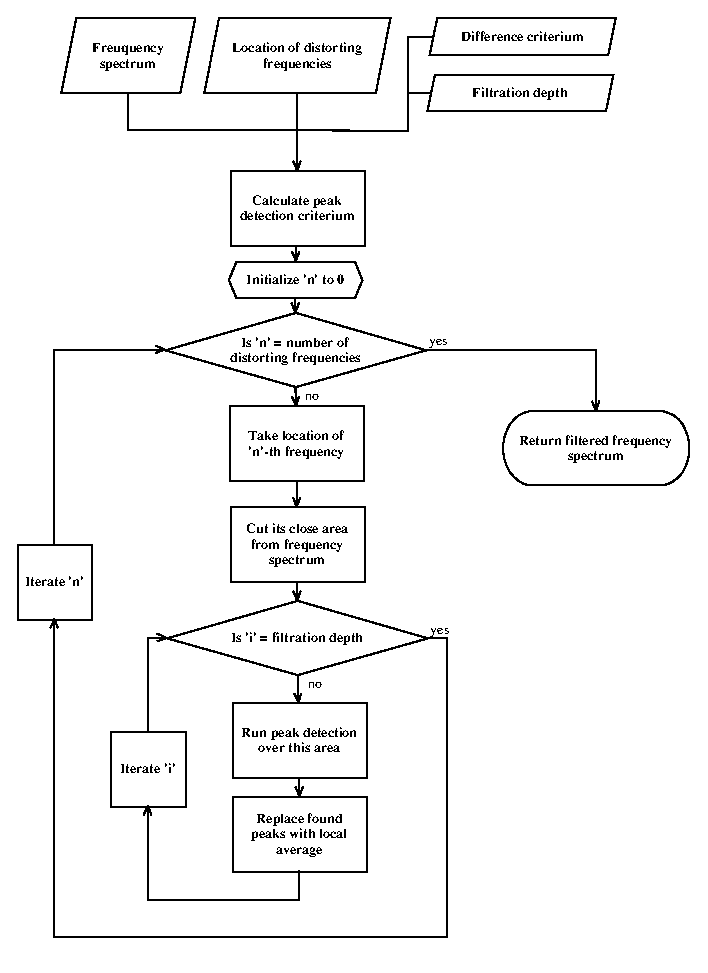
\includegraphics[width=0.75\textwidth]{frequencyFiltration.eps}
	\caption{Flowchart diagram of applied frequency filtration}
	\label{fig:frequencyFiltration}
\end{figure}

Inputs to the function are:
\begin{itemize}
	\setlength{\itemsep}{5pt}
	\item Distorted frequency spectrum.
	\item Known approximate locations of distorting frequencies.
\end{itemize}
And parameters for the frequency filtration:
\begin{itemize}
	\setlength{\itemsep}{5pt}
	\item Difference criterium.
	\item Filtration depth.
\end{itemize}
The difference criterium is used to calculate parameter $\delta$ for peak detection. This is done according to the formula \ref{eq:deltaCalculation}.
\begin{equation} \label{eq:deltaCalculation}
\delta = \sigma \cdot \textit{difference criterium},
\end{equation}
where $\sigma$ is standard deviation of given frequency spectrum.
Filtration depth is parameter determining how many times is the peak detection performed over the same areas. Executing peak detection several times can help to refine the result since it improves filtration of wider peaks. The parameters were empirically set as $\textit{difference criterium}=1.5$ and $\textit{filter depth} = 2$ for all the stages.

\subsubsection{IFFT}
After the filtration in frequency domain we have to obtain the corresponding signal in time domain. For this purpose we use inverse fourier transform (see \ref{sec:FFT}). Implementation for microcontroller is available in the DSP libraries for ARM. Specficially, for IFFT we use the same function as for FFT with difference that the flag determining whether forward or inverse Fourier transfourm should be calculated, is set. This means using function \textit{arm\_rfft\_fast\_f32} with length of IFFT 1024.

\subsubsection{CV Calculation}
Last step of every branch is calculation of coefficient of variation (see chapter XXX). This coefficient is widely used in describing quality of textile fibers. Its percentual value the CV\% can be calculated as follows in \ref{eq:CVCalculation}:

\begin{equation} \label{eq:CVCalculation}
CV\% = \frac{\sigma}{\mu} \cdot 100
\end{equation}

Since we have obtained filtered signal from the IFFT, it is easy to calculate the resulting CV value. This is done for each branch (i.e. wavelength), therefore, there is 12 CV values.

\subsection{Variance-Length Curve}
The output of the quality sensor for the sliver is required to be a variance length curve (see chapter XXX). This curve is composed of the results of the processing branches, therefore, of the CV\% values. These values are concatenated in a vector that represents values on the y-axis of the curve. The x-axis contains values of the corresponding wavelengths (see table \ref{tab:Wavelengths}). Since every wavelength value is the double of the previous one, it is appropriate to use logarithmic scale on the x-axis. Example of the result in form of the variance-length curve is shown in figure \ref{fig:VLC_example11}. This particular curve was calculated on data set of high quality sliver without any simulated defect (more information in chapter XXX). 

\begin{figure}[h]
	\centering
	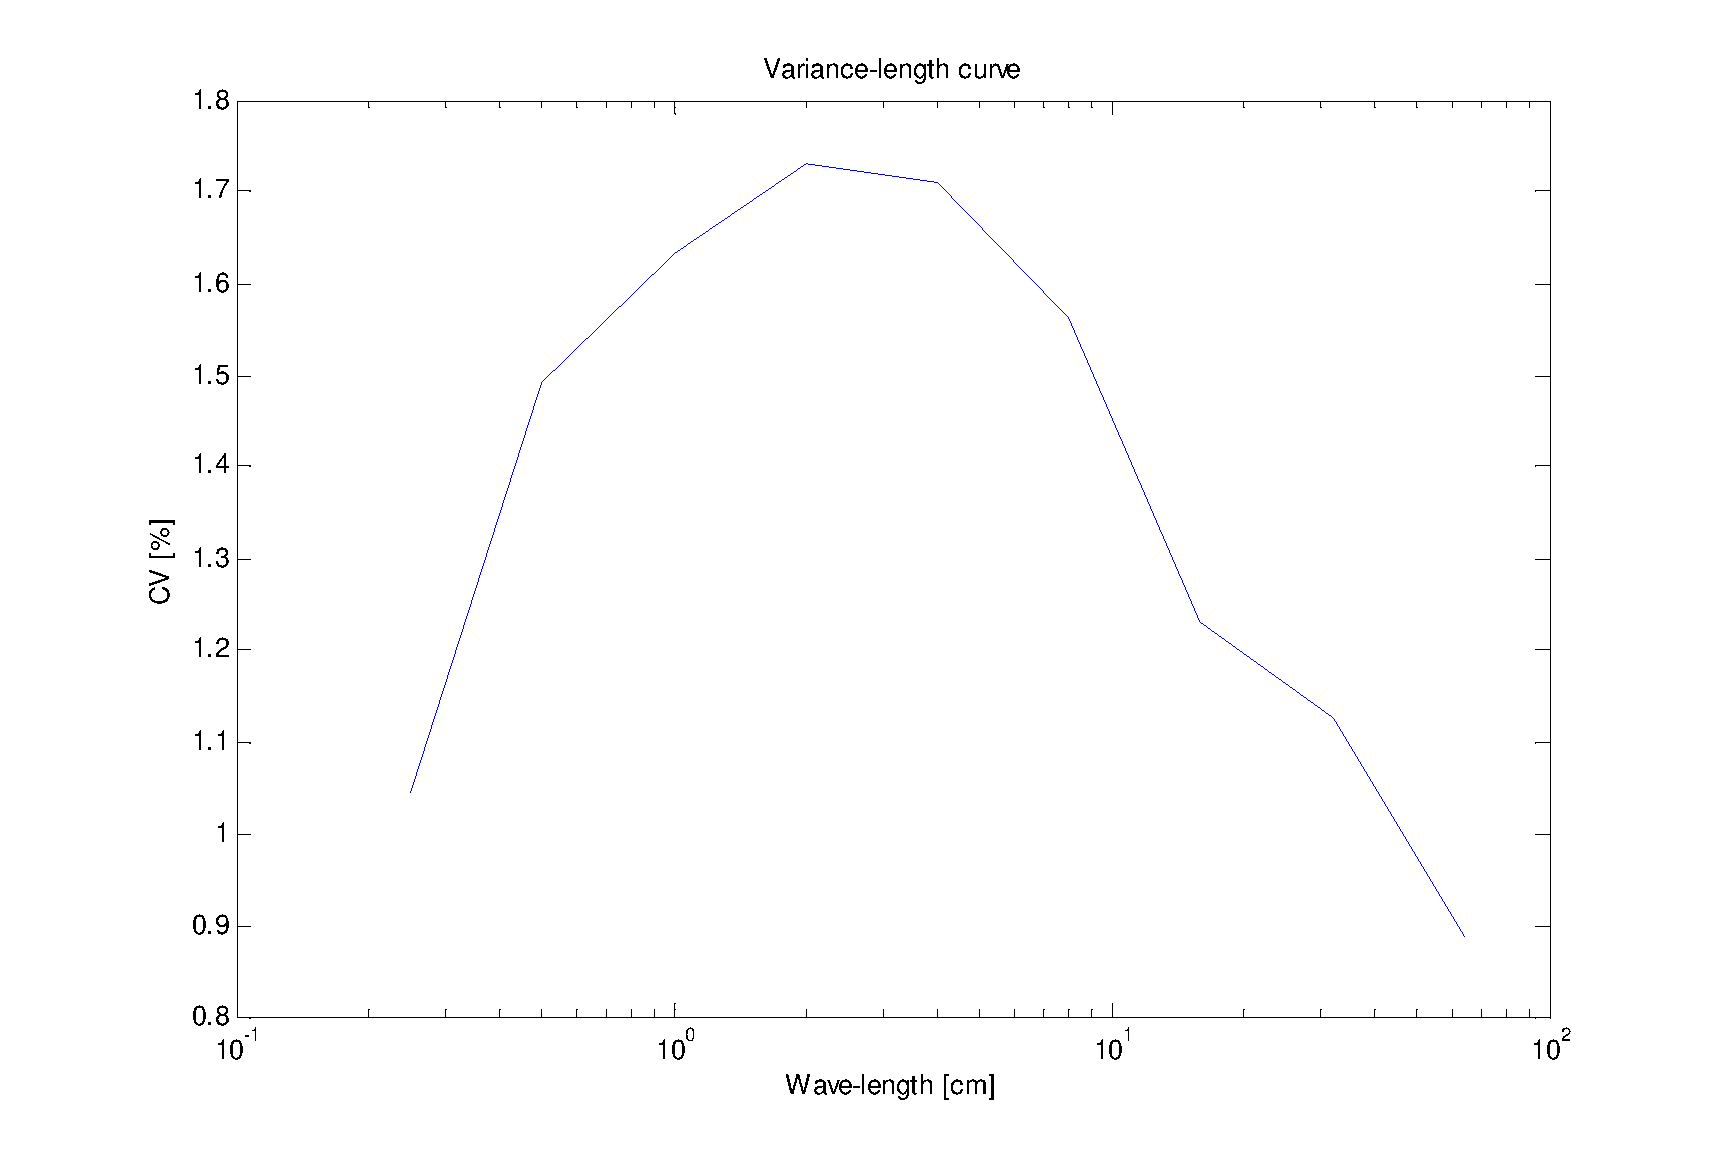
\includegraphics[width=1.0\textwidth]{full_VLC_11.eps}
	\caption{Variance-length curve - the output of the algorithm}
	\label{fig:VLC_example11}
\end{figure}

\subsection{Measurement and Testing}
\label{sec:MeasurmentAndTesting}
For the purpose of testing the algorithm new data set has to be created. This was obtain in Swiss laboratories of Rieter where I personally conducted measurement on the prototype of the device. The prototype was connected to the sensor which was placed inside combing machine (see chapter \ref{sec:Combing}). In concrete, the comber type was \textit{E86} developed by Rieter and its technical description is in \cite{cite:ComberE86}. The sensor that was used for the measurement of the diameter was Baumer Inductive Sensor S35A (for details see chapter \ref{sec:Sensors}).

This prototype had to be specifically modified to perform the measurements. Hardware remained the same but change was made in the software to meet the goals of measurement. The device didn't evaulated quality of the sliver but instead sent the measured data to the service computer over the USART peripheral. Specifically sample is taken by an ADC from the pin connected to a sensor, then the sample is propagated to the USART interface by DMA. The USART is connected to the computer which stores the data on a hard-drive. The prototype of the device is shown in figure \ref{fig:cvBox_covered}.
\begin{figure}[h]
	\centering
	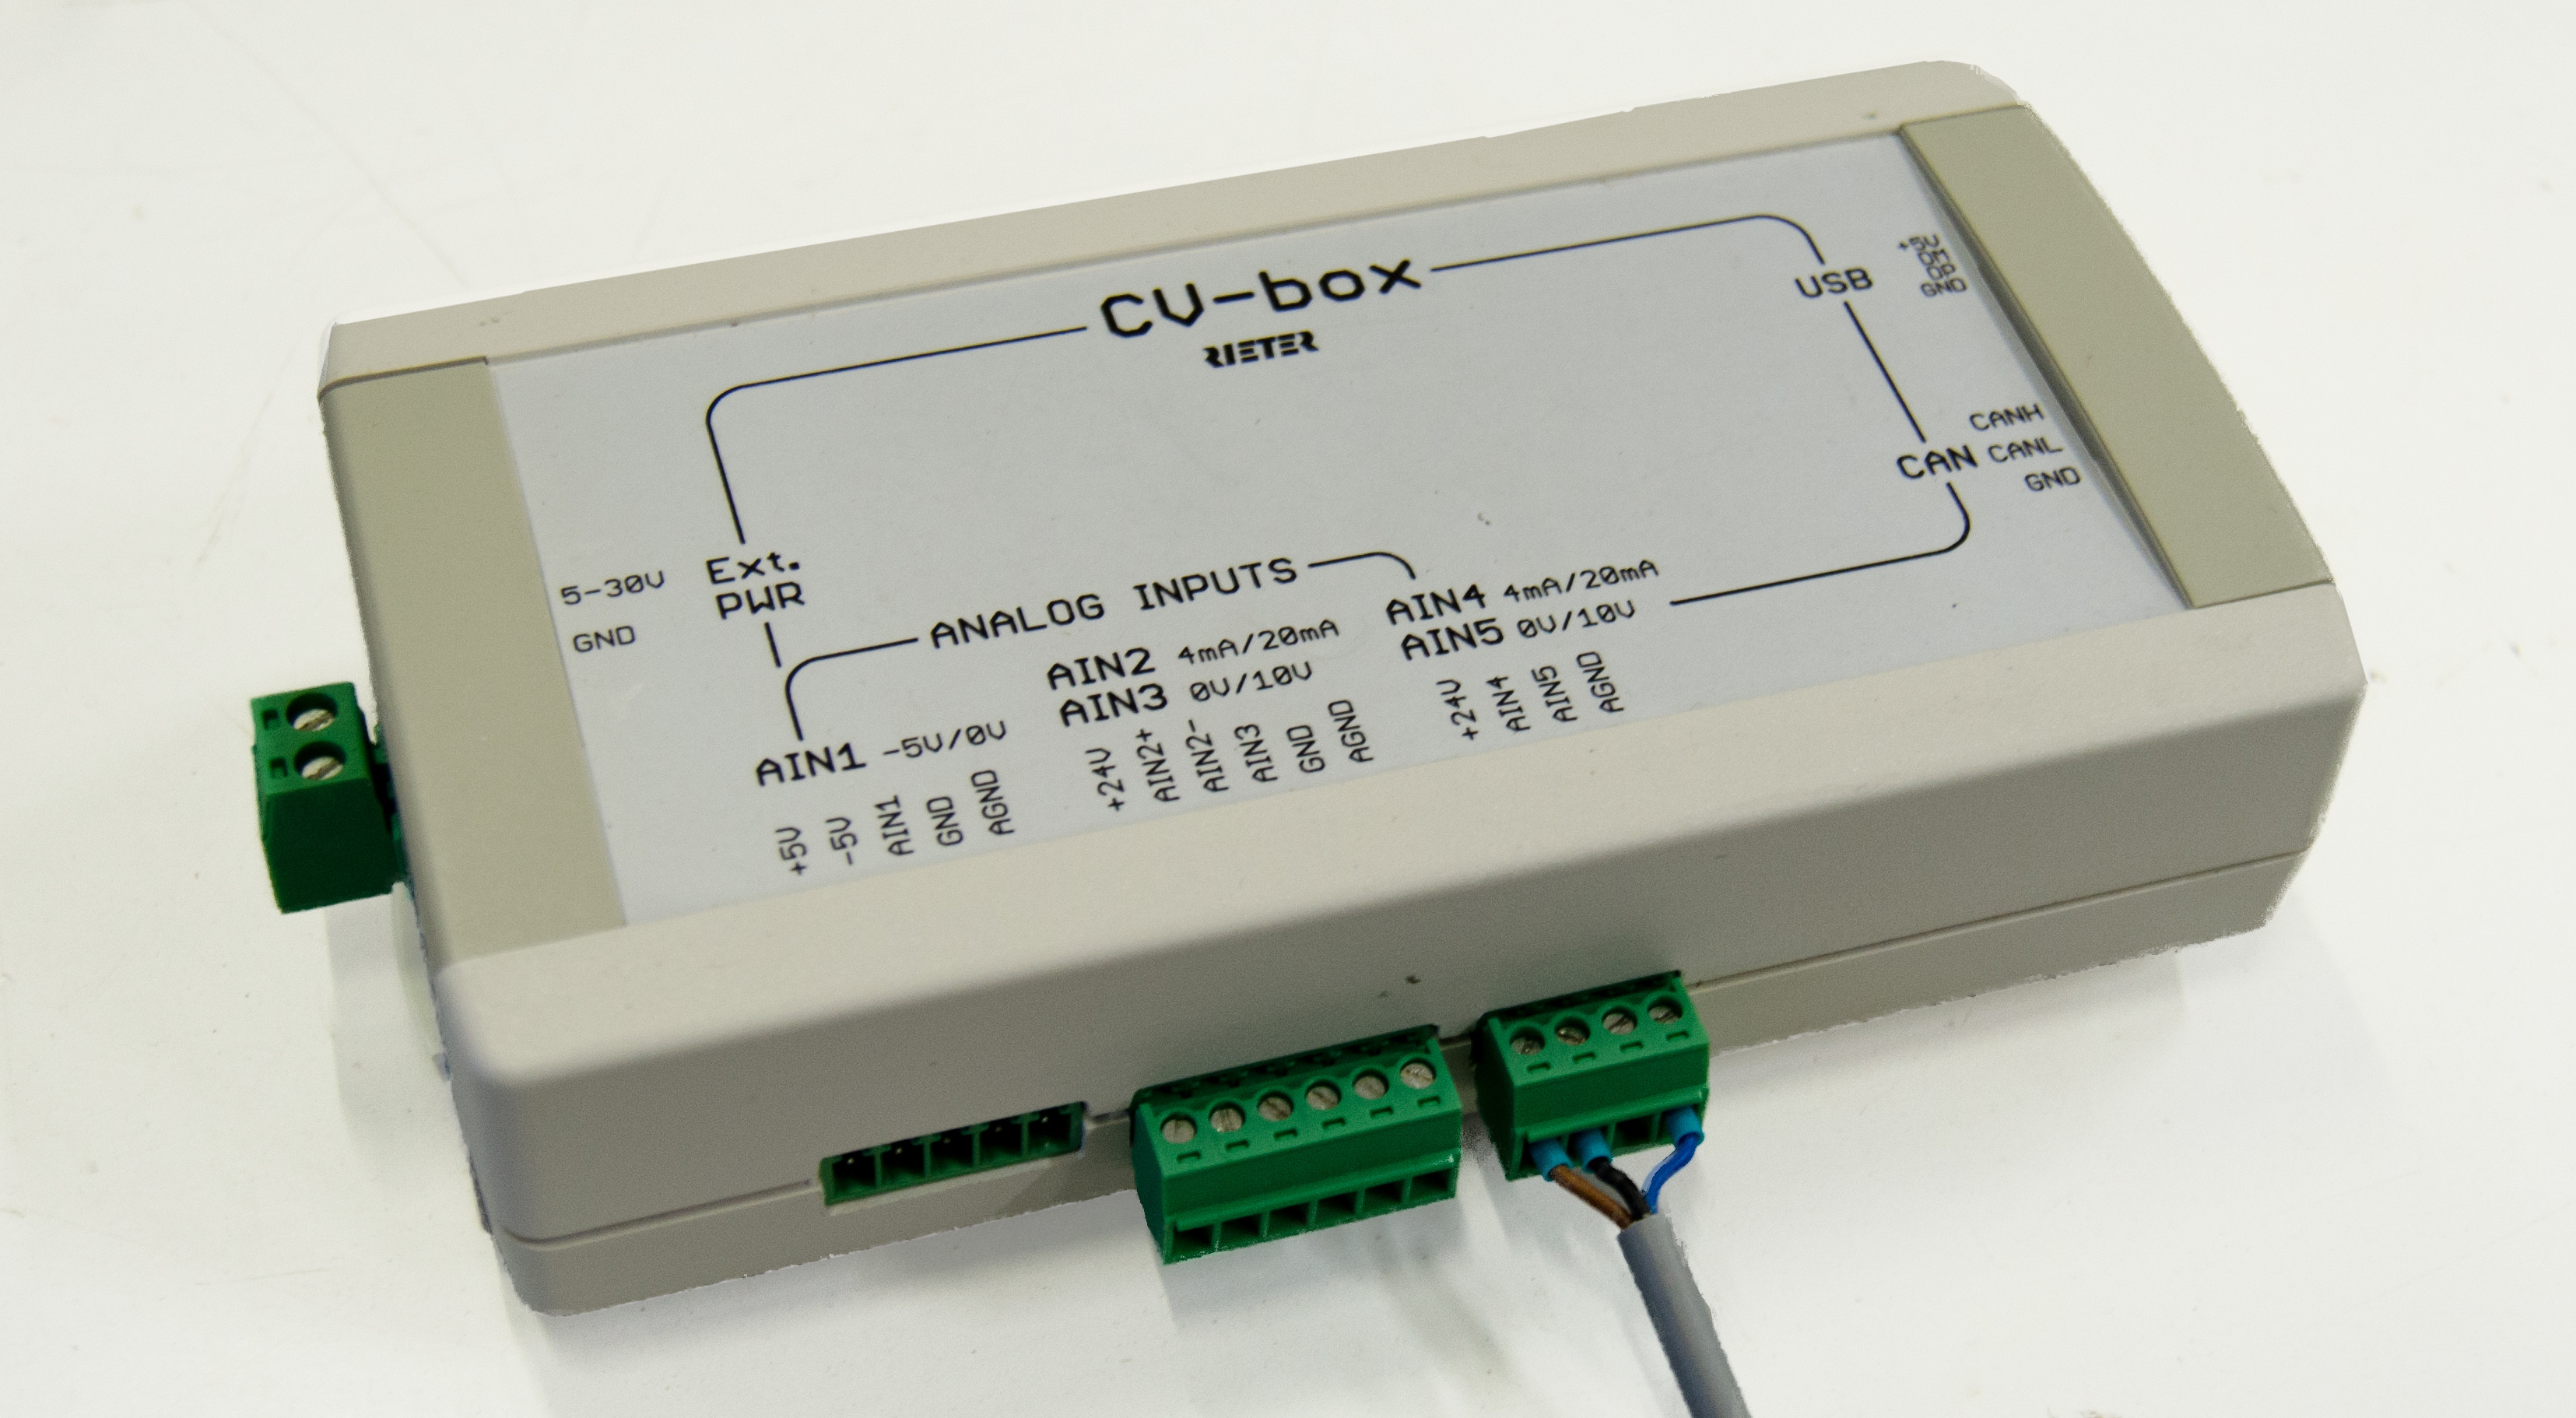
\includegraphics[width=0.75\textwidth]{cvBox_covered.jpg}
	\caption{Prototype of the device}
	\label{fig:cvBox_covered}
\end{figure}

To obtain as much information as possible, the sampling frequency is needed to be set to the feasible maximum. This maximum is strictly dependent on a number of sensors used, since the more samples has to be send in each cycle. And the sending has to be executed in a time lesser than a sampling period. This is, of course, limited by speed of the USART which was set to the maximum speed of $115200 b/s$. Maximum allowed sampling frequencies where set as shown in table \ref{tab:possibleFs}.
\begin{table}[htbp]
	\centering
	\caption{Maximum possible sampling frequencies}
	\begin{tabular}{cccccc}
		\toprule
		Number of Sensors	 & 1 & 2 & 3 & 4 & 5 \\
		\midrule
		Sampling Frequency [Hz]  & 6500  & 4400   & 3300 & 2600   & 2200  \\
		
		\bottomrule
	\end{tabular}%
	\label{tab:possibleFs}%
\end{table}%

\subsubsection{Measurement Application}
To control and set the properties of measurement and also to store measured values an application for service computer was implemented. This application was written in Java. Its main purpose relays in connecting the device using USART, receiving measured samples and logging them into a file. As an auxiliary action it is also capable of sending required settings to the microcontroller and starting or stopping the measurement. Graphical user interface of the application is shown in figure \ref{fig:gui_APP}.
\begin{figure}[h]
	\centering
	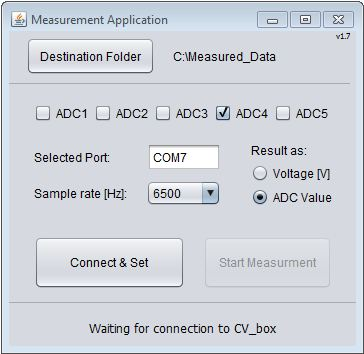
\includegraphics[width=0.5\textwidth]{Measurement_app.JPG}
	\caption{Measurement application - graphical user interface}
	\label{fig:gui_APP}
\end{figure}

The application allows to pick sensors that should be used by enabling corresponding ADC pins (1 to 5). Another options to set is sampling frequency. This can be done by choosing from several values offered by graphical user interface. The values offered are changed according to number of ADC pins enabled and only sampling frequencies smaller than the corresponding one in table \ref{tab:possibleFs} are available. These settings are send to the microcontroller after button \textit{Connect \& Set} is applied. The microcontroller will parse these values and use them in initialization of the ADC peripheral.
Another options are available for setting in the application that are designated only as parameters for the application itself. It is possible to set a format of the output to either representation in Volts or in unconverted output values of ADC, which ranges between 0 to 4095.
The data that are read over USART are being continuously logged in a file from the moment the \textit{Start Measurement} is clicked until \textit{Stop Measurement} is pressed. This means that a length of the measured signal is unknown, thus, no buffering can be used. The data has to be written into file in sample by sample technique. An action diagram of the application is shown in figure XXX.


\subsubsection{Measurement}
\label{sec:measurement}
To test if algorithm can properly calculate variance-length curve measurements had to be made with slivers of different qualities. This allows to compare the curve of a high quality sliver and a sliver that contains defects. The variance-length curves of the two should clearly distinguishable. Unfortunately, no sliver with defect is easy to obtain as defects are not known until the sliver is being processed. 

The solution was found by artificially simulating defects. This could be done by incorrect settings of the pressures of the sliver holder in combing machine. The holder can be set by two pressures: $p_{left}$ and $p_{right}$. If these pressures are set to inappropriate values, the sliver gets defected with periodical errors. As an inappropriate values can be considered either too high or too uneven levels of pressures. Image of how does the sliver affects the sliver is shown in figure XXX.
Using this method of simulating defects 6 data sets were measured. Their properties are listed in table \ref{tab:measuredData}.
\begin{table}[htbp]
	\centering
	\caption{Measured data and their properties}
	\begin{tabular}{cccc}
		\toprule
		Dataset ID & $p_{left}$ [bar] & $p_{right}$ [bar] & Visual Sliver Quality \\
		\midrule
		1     & 1.85  & 2.1   & Very Poor \\
		2     & 1.7   & 2.1   & Poor \\
		3     & 1.7   & 1.3   & Good \\
		4     & 1.9   & 1.8   & Good \\
		5     & 1.5   & 1.6   & Excellent \\
		6     & -     & -     & No Sliver \\
		\bottomrule
	\end{tabular}%
	\label{tab:measuredData}%
\end{table}%
All the datasets were measured with the same sliver speed $v_s=30cm/s$. This is important for the calculation of the wavelengths, which is described in section \ref{sec:WavelengthSpecification}).
The dataset 6 is a special case where no sliver was placed into the combing machine. This was for the purpose of measuring distorting frequencies caused by vibrations of the gears (see chapter \ref{sec:spectrumFiltration}). Without a sliver as input only these frequencies are measured by the sensor.

\subsection{Algorithm Results}
The algorithm was tested on the data described in table \ref{tab:measuredData}. To meet the requirements for the device, a result should have following properties:
\begin{itemize}
	\setlength{\itemsep}{5pt}
	\item Result should have form of variance-length curve.
	\item Quality of a sliver should be recognizable from the result.
\end{itemize}

Slivers with good visual quality are expected to have lower CV\% values than the one with a bad visual quality. This expectation is based on how is the CV\% calculated (see \ref{sec:CoefficientOfvariation}). Another expectation is that the variance length should be decreasing for the longer wavelengths, unless there is a defect on the corresponding wavelength in the sliver.

Variance-length curve calculated on the dataset 5 (see section \ref{sec:measurement}) is shown in the figure \ref{fig:sub_dataset5}. Accordingly to the table \ref{tab:measuredData}, we can state that the sliver in this dataset is of very good visual quality and it was with low amount of simulated defects. For comparison, the sliver with worse visual quality from dataset 2 is shown in figure \ref{fig:sub_dataset2}. From the \ref{fig:vlc_curves} it is observable that the sliver in dataset 5 has lower CV\% values for all of the wavelengths than sliver in dataset 2. Thus, it has smaller variance and we can state that the quality of the sliver is higher. This observation corresponds to the visual quality of th slivers.
It can also be seen that the shapes of variance-length curves are very similar in both of them. This is due to the fact that used slivers are, in fact the same one and only difference is in added simulated defects. These defects are significant in wavelengths smaller than $\lambda=16cm$ after which the CV\% values are on equivalent level. If it would be possible to simulate defect only on a specific wavelength, it would be distinguishable in charts as a peak. 

\begin{figure}
	\centering
	\begin{subfigure}{0.5\textwidth}
		\centering
		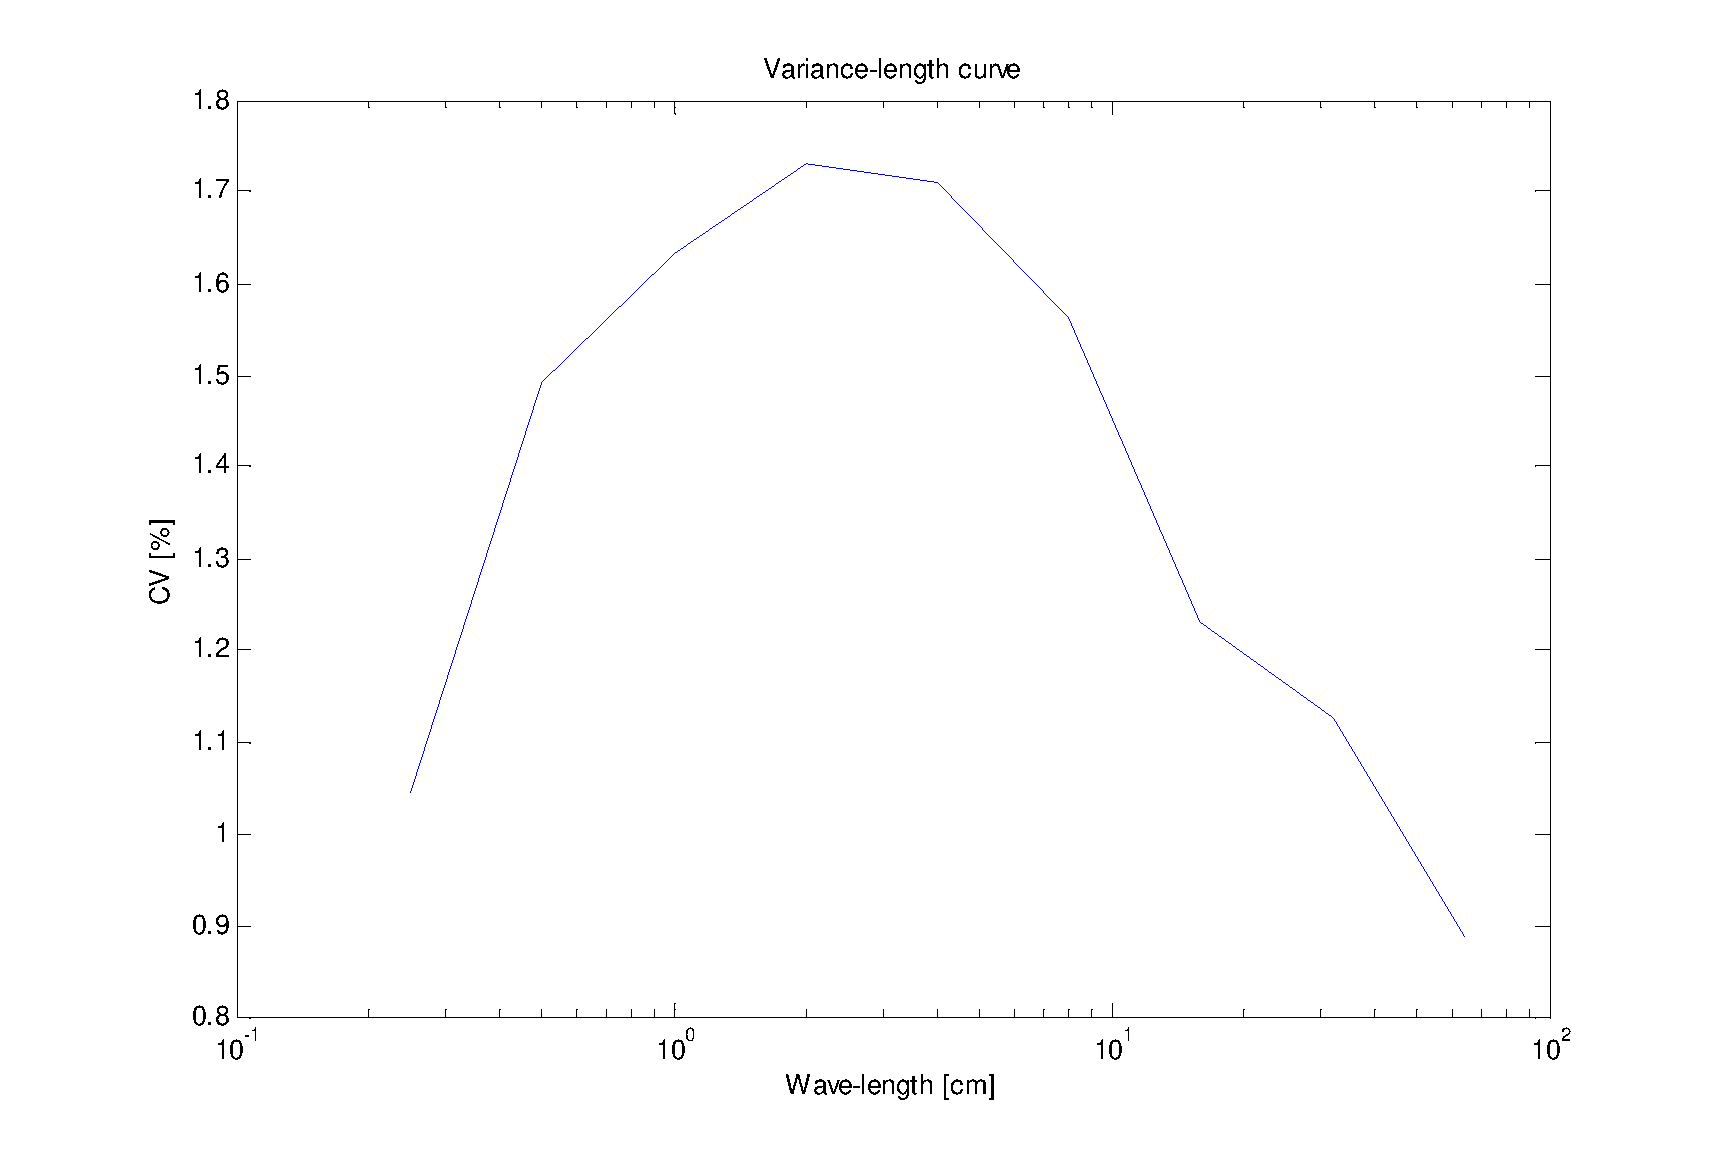
\includegraphics[width=1.0\linewidth]{full_VLC_11.eps}
		\caption{Dataset 5}
		\label{fig:sub_dataset5}
	\end{subfigure}%
	\begin{subfigure}{0.5\textwidth}
		\centering
		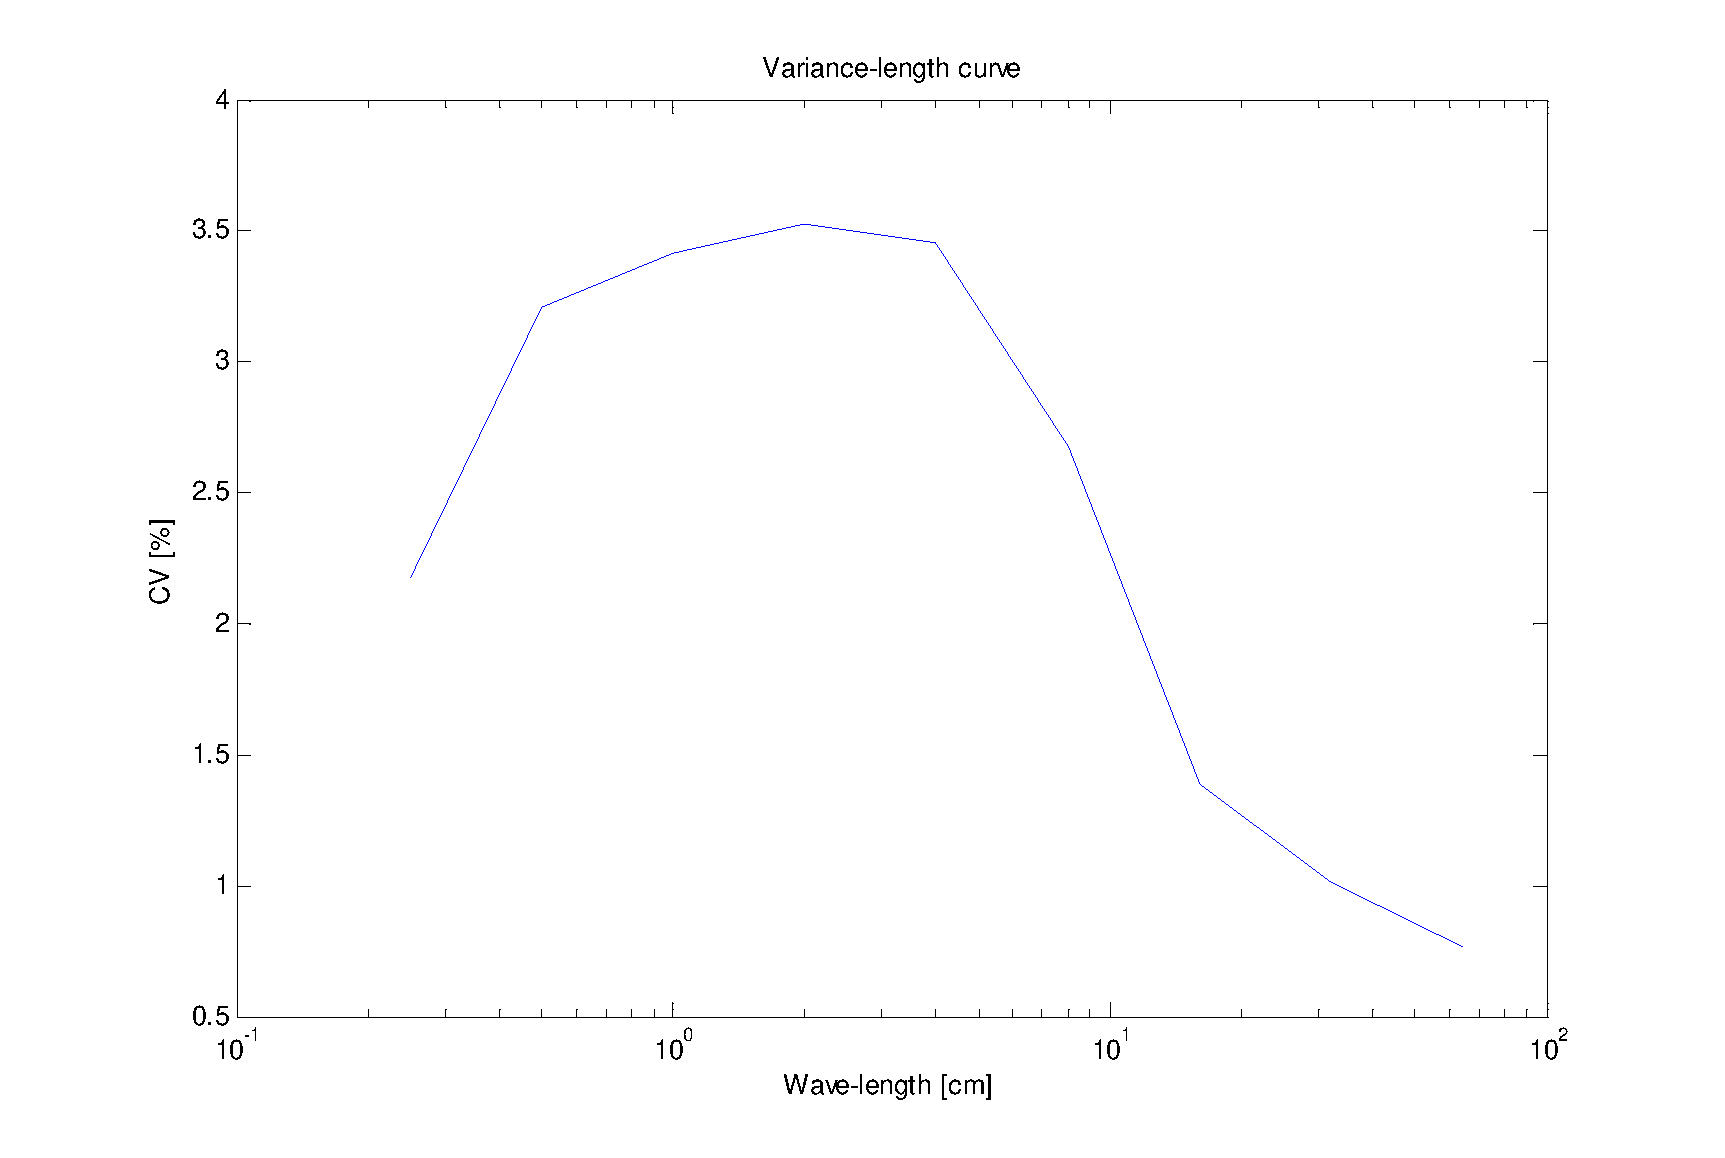
\includegraphics[width=1.0\linewidth]{full_VLC_6.eps}
		\caption{Dataset 2}
		\label{fig:sub_dataset2}
	\end{subfigure}
	\caption{Variance-length curves}
	\label{fig:vlc_curves}
\end{figure}

Plot of results for the datasets 3-5 is shown in figure \ref{fig:VLC_3_4_5}. All of these datasets were measured with slivers whose visual quality was rated as good or excellent (in case of dataset 5). This comparison can be considered as a prove that the algorithm is capable of distinguishing slivers of very similar quality. This can be stated because the dataset 5 appears in the chart as superior in terms of quality, which corresponds with its visual quality rating \textit{excellent}. Visual check of the slivers in datasets 3 and 4 could not determine which has better quality as they were both rated \textit{good}.But it is clearly determinable from variance-length curve that dataset 4 has better quality.

It is interesting to observe that although the dataset 5 has the best quality as determined by visual check and variance-length curve, there is an exception to this statement on wavelength $\lambda=32cm$. From the plot \ref{fig:VLC_3_4_5} it can be seen as little peak. This is especially visible in comparison with the dataset 4, which doesn't contain this defect. This tells us that there is small defect on this particular wavelength. And even though the defect is not visible in the sliver, it can cause a visible periodic error in final product.
\begin{figure}[h]
	\centering
	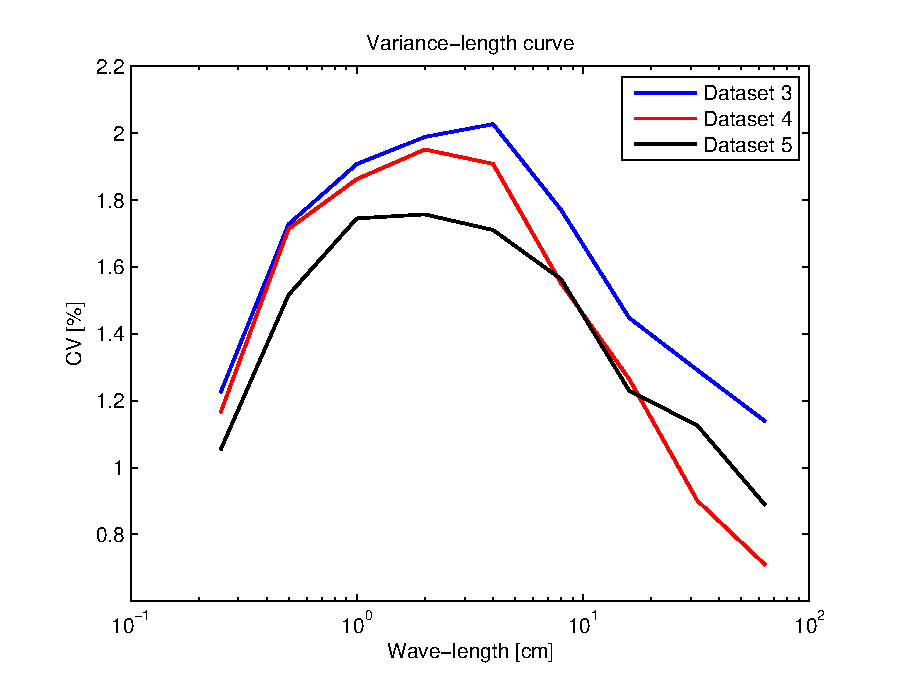
\includegraphics[width=1.0\textwidth]{VLC_curves_3_4_5.eps}
	\caption{Variance length curves - comparison of datasets with slivers of high quality}
	\label{fig:VLC_3_4_5}
\end{figure}

Comparison of the results of the algorithm on all datasets 1-5 are shown in an figure \ref{fig:VLC_all}.
\begin{figure}[h]
	\centering
	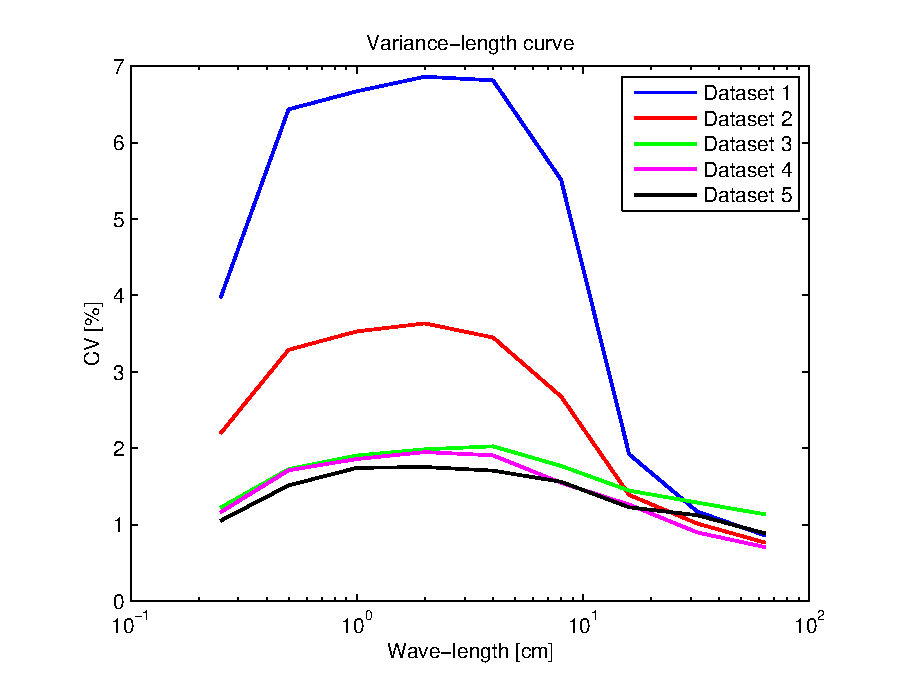
\includegraphics[width=1.0\textwidth]{VLC_allCurves.eps}
	\caption{Variance length curves - comparison of all datasets}
	\label{fig:VLC_all}
\end{figure}

\section{Yarn Quality Analysis}
The yarn quality analysis requires only software algorithm and no additional hardware. This is because measurement of a yarn diameter is done by a row camera sensor that is connected to processing board which was already developed in Rieter. Processing board has CAN interface that sends values of diameters to the microcontroller. 

Therefore, in this part of the project, the only input we consider are values of diameter send over CAN. This determines the project as software system with main requirements and features defined as follows:
\begin{itemize}
	\setlength{\itemsep}{5pt}
	\item The system shall receive yarn diameter values and process them in a way that yields spectrogram values as output.
	\item The system shall be able to run on ARM microcontrollers STM32F4xx series.
	\item The system shall be written only as a software library.
\end{itemize}

\subsection{Hardware}
Because the system is required as a software library only then no hardware is specifically necessary. But for testing purposes was used microcontroller STM32F407. This ensures that the algorithm meets the requirement that algorithm shall run on ARM microcontrollers STM32F4xx series.
\subsubsection{Control Unit}
\label{sec:microControllerYarn}
Only part of the hardware is control unit STM32F407VG. This microprocessor is used in developement kit \textit{STM32F4 Discovery}.
The microcontroller is based on ARM Cortex-M4 technology with ARMv7 architecture \ref{sec:ARM_M3}. Maximal operation frequency is $168 MHz$ at which gives $210 DMIPS$ (Dhrystone benchmark). The most important features and peripherals of this microcontroller are:
\begin{itemize}
	\setlength{\itemsep}{5pt}
	\item ARM 32-bit Cortex-M4, 168 MHz,
	\item 1 MB of Flash memory,
	\item 192 kB of SRAM,
	\item SWD and JTAG debug interface,
	\item 17 Timers and 3 ADC,
	\item Communication interfaces such as USART, CAN, SPI etc.
\end{itemize}	

\subsection{Algorithm for Yarn Quality Analysis}
Digital signal processing algorithm for evaluation of yarn quality is based on the idea described in \cite{cite:1}. Its implementation is similar to the algorithm for sliver quality analysis (see chapter \ref{algorithmForSliver}) but has certain important differences. First difference is caused by distinct required output of the algorithm. For a sliver it was variance-length curve, but for a yarn it is spectrogram (see chapter XXX). This modifies some of the software components used for slivers.

The block diagram (shown in figure XXX) of the software remains the same with two exception:
\begin{itemize}
	\setlength{\itemsep}{5pt}
	\item Output of each processing branch is partial spectrogram. 
	\item Final block is compilation of full spectrogram.
\end{itemize}
\begin{figure}[h]
	\centering
	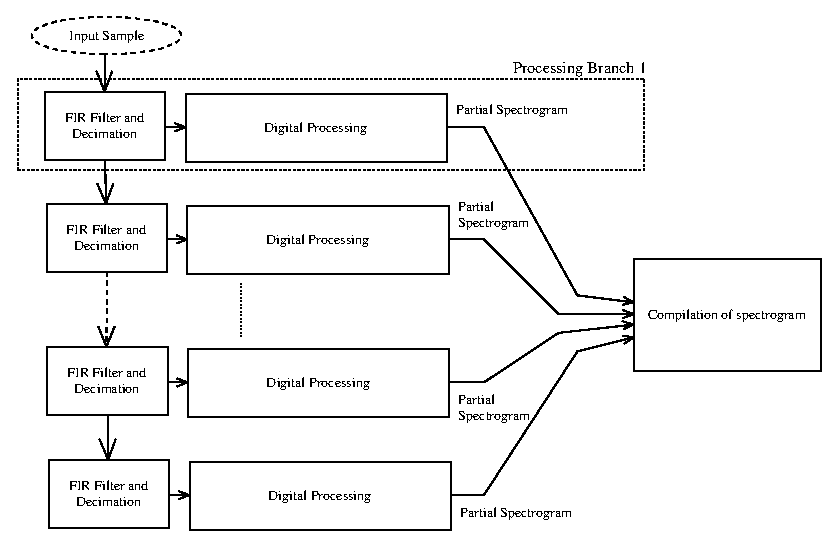
\includegraphics[width=1.0\textwidth]{system_overview_yarn.eps}
	\caption{Software Architecture Overview - Yarn Analysis}
	\label{fig:software_overview_yarn}
\end{figure}

To obtain spectrogram it is necessary to calculate frequency spectrum. But it is not possible to store sufficient amount of samples in microcontroller to determine frequency spectrum of very low frequencies (i.e. high wavelengths) with adequate resolution. For this reason the multi-rate analysis needs to be implemented. This uses decimation and appropriate filtration to obtain signals who contain only frequencies for praticular wavelengths. Frequency spectrum is calculated by FFT from these signals and its components are used for calculation of spectrogram. Processed are the same wavelengths as in the sliver analysis, which are described in table \ref{tab:Wavelengths}.

\subsection{Processing Branch}
In processing branch for yarn quality analysis signal is first filtered by FIR filter that is described in \ref{FIR filter}. This prevents aliasing that could occur after downsampling, which is done as the next step of processing. This filtration and downsampling is executed sample-to-sample. After each sample is passes the decimation it is buffered for calculation of FFT. Also, it is used as input sample in the next processing branch. The block software diagram of each processing branch is in figure \ref{fig:singleBranch_yarn}.
\begin{figure}[h]
	\centering
	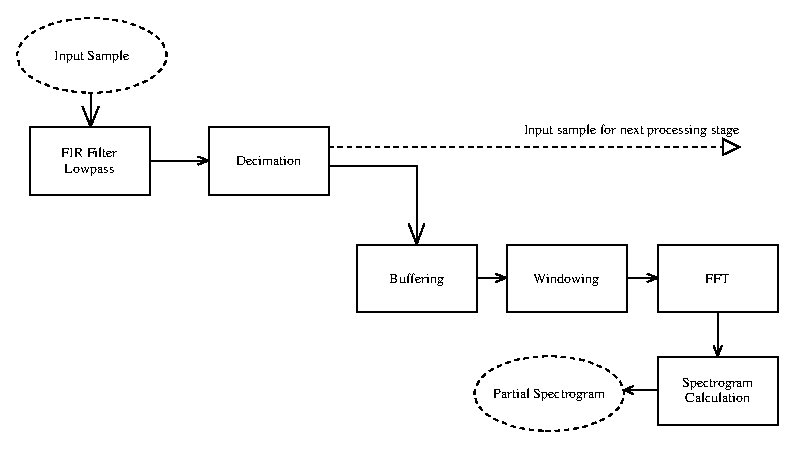
\includegraphics[width=1.0\textwidth]{yarn_singleBranch.eps}
	\caption{Component Diagram of Individual Processing Branch - Yarn Analysis}
	\label{fig:singleBranch_yarn}
\end{figure}



\subsection{Flowchart Diagram}
\section{Description of Designed System}
\subsection{Block Diagram}
\section{Implementation of Software}
\subsection{Filtration}
%For practical spectral analysis like this, we deal with finite duration discrete-time signals, whose spectrum is given by the DTFT. The N-point FFT is merely used to evaluate samples of the DTFT at N equally spaced frequencies omega=2pik/N, 0 leq n leq N-1. Therefore we needed to use good window (like Hann) and oversample DTFT.
\subsection{Detection of Defects}
\subsection{Automatic Evaulation}
\subsection{Example of Designed Application}
\section{Implementation of Hardware}
\subsection{Electronic Circuits Design}
\subsection{Description of possible sensors}
\subsection{Designed Prototype}
\chapter{Conclusions}


\medskip

\begin{proof}\begin{enumerate} \item[8] Bla \item Blo \end{enumerate} \end{proof}

\appendix

\printindex

\appendix

%\bibliographystyle{amsalpha}
\bibliographystyle{siam}
\bibliography{ctuDIP_biblio}

\ctutemplate{specification.as.chapter}

\end{document}